\documentclass[10pt,letterpaper,final]{article}

\usepackage[spanish]{babel}
\spanishdecimal{.}

% \usepackage[left=2cm, rigth=1.5cm, top=1.5cm, bottom=1.5cm]{geometry}

% Esta linea tenia un error debiera ser 'right' en lugar de 'rigth'.
\usepackage[left=2cm, right=1.5cm, top=1.5cm, bottom=1.5cm]{geometry}
\usepackage[utf8]{inputenc}
\usepackage{amsmath}
\usepackage{amsfonts}
\usepackage{amssymb}
\usepackage{graphicx}
\usepackage{kpfonts}
\usepackage{tabularx}
\usepackage{hyperref}
\usepackage{natbib}
\usepackage{colortbl}
\usepackage{tikz}
\usepackage{ragged2e}
\usepackage{caption}
\usepackage{subcaption} % Paquete para justificar el texto
%gantt chart
\usepackage{pgfgantt}


%\title{Estimación de la posición relativa al estacionamiento de un vehículo mediante cámaras y sensores para parqueo automático en simulación}
\title{Estimación de la pose de un vehículo mediante cámaras y sensores para estacionamiento automático en simulación}
%\author{Rubén Martínez González}
%\tutor{Dr. Arturo Espinosa Romero}
\date{Enero 2025}

\begin{document}

    \maketitle
    \begin{minipage}[t]{0.45\textwidth}
        \centering
        \rule{6cm}{0.4pt} \\ % Línea para firma
        Autor: Ing. Rubén Martínez González
    \end{minipage}
    \hfill
    \begin{minipage}[t]{0.45\textwidth}
        \centering
        \rule{6cm}{0.4pt} \\ % Línea para firma
        Asesor: Dr. Arturo Espinosa Romero
    \end{minipage}
    \clearpage

    \section*{Introducción}
    \noindent
El avance continuo en la tecnología de vehículos autónomos representa un logro significativo en la revolución del transporte.
Existe la necesidad de desarrollar sistemas ``inteligentes'' que permitan a estos vehículos aprender a conducir de manera autónoma y,
al mismo tiempo, detectar posibles colisiones y reaccionar de manera similar a como lo haría un conductor humano.
La convergencia de la inteligencia artificial, la visión computacional y los sistemas de control ha generado una nueva era en la movilidad,
desafiando y redefiniendo las fronteras de la conducción convencional.
Si bien los avances en la conducción autónoma han sido significativos, la detección y respuesta a
situaciones de peligro, como colisiones inminentes, siguen siendo un desafío complejo.\\ \newline
En este contexto, este trabajo se centra en el desarrollo de un sistema de detección y evasión de colisiones basado en visión computacional.
Para lograr este desarrollo se conformará un entorno simulado que refleje el escenario de conducción de un vehículo,
y mediante algoritmos de visión computacional se analizará la información proveniente de cámaras y sensores.
Con el procesamiento de estos datos se podrá modelar el medio que rodea al vehículo, lo que posibilitará
el desarrollo de estrategias de detección y evasión de colisiones en diferentes situaciones de manejo.
Una vez que se ha realizado el procesamiento exhaustivo de los datos provenientes de cámaras y sensores mediante técnicas de visión computacional,
se plantea la posibilidad de emplear algoritmos de aprendizaje por refuerzo.
Los algoritmos de aprendizaje por refuerzo, al recibir estos datos procesados como entrada, tienen la capacidad de aprender de manera progresiva
a tomar decisiones inteligentes en tiempo real.
Aprovechando la retroalimentación proporcionada por el entorno, estos algoritmos pueden mejorar continuamente su capacidad para reaccionar y evitar colisiones.\\ \newline
La seguridad en la carretera y la confianza del público en esta tecnología dependen en gran medida de la capacidad
de los vehículos autónomos para enfrentar situaciones de tráfico de manera eficiente y segura.
Esta investigación busca abordar esta problemática crítica, avanzando hacia el escenario en el que los vehículos autónomos
sean capaces de igualar e incluso superar las habilidades de conducción humana en términos de detección y respuesta
a situaciones de colisión.
    \clearpage

    \section*{Contexto y problemática}
    \noindent
%    problemas en los estacionamientos
Los estacionamientos son imprescindibles en la vía urbana, ya que permiten a los conductores estacionar sus vehículos
de manera segura y eficiente. Sin embargo, el proceso de estacionamiento puede ser complicado y estresante,
especialmente en áreas congestionadas con espacio limitado y visibilidad reducida.
Factores como la falta de espacio, la presencia de obstáculos y la poca visibilidad para el conductor ocasionan
dificultades al estacionar un vehículo, lo que puede aumentar el riesgo de colisiones y daños al vehículo.
\\
%   se han logrado sistemas de asistencia al conductor
En la actualidad, la búsqueda de soluciones para mejorar la eficiencia y seguridad en el desplazamiento vehicular
ha llevado al desarrollo de sistemas avanzados de asistencia al conductor.
Entre estos sistemas, el estacionamiento automático ha ganado relevancia como una función que puede contribuir
a reducir los riesgos asociados con el estacionamiento en entornos urbanos congestionados.
\\
%   problemas de sistemas de estacionamiento automático
Sin embargo, el desarrollo de sistemas de estacionamiento automático presenta desafíos significativos,
especialmente en lo que respecta a la estimación de la posición del vehículo con respecto al espacio de estacionamiento.
El cálculo incorrecto de esta posición puede resultar en maniobras de estacionamiento inseguras o peligrosas,
especialmente en entornos donde el espacio de estacionamiento es limitado o con poca visibilidad para el conductor.
\\
%   necesidad de sistemas de asistencia al conductor más autónomos
En este contexto, continua la necesidad de desarrollar soluciones de utilidad para que los sistemas de asistencia al conductor
sean cada vez más autosuficientes y no dependan de la intervención limitada del conductor.
\\
%   en que consiste la investigación
Esta investigación se enfoca en poder estimar la posición de un vehículo con respecto a su espacio de estacionamiento
utilizando cámaras y sensores y utilizar esta posición estimada para lograr un sistema de estacionamiento automático en simulación.
    \clearpage

    \section*{Preguntas de investigación}
    \begin{itemize}
        \item ¿Cómo se puede representar la posición de un vehículo con respecto a su espacio de estacionamiento?
        \item ¿Cómo se puede estimar esta posición utilizando las cámaras y sensores del vehículo?
        \item ¿Cómo usar esta posición estimada para que el vehículo se estacione automáticamente?
    \end{itemize}

    \section*{Hipótesis}
    \noindent
    ``Estimando la posición relativa al estacionamiento de un vehículo mediante cámaras y sensores,
    y utilizando esta posición, se puede lograr un sistema de parqueo automático en simulación.''

    \section*{Objetivos}
    \noindent{Objetivo general:}
\newline
\noindent Desarrollar un sistema de estimación de la posición relativa al estacionamiento de un vehículo mediante cámaras y sensores para parqueo automático.
\newline
\newline
\noindent{Objetivos específicos:}
\begin{itemize}
    \item Modelar un ambiente de simulación de un vehículo y estacionamiento.
    \item Obtener datos de los sensores del vehiculo en simulación.
    \item Interpretar los datos de los sensores mediante técnicas de visión computacional.
    \item Procesar los datos y estimar la posición del vehículo con respecto al estacionamiento.
    \item Utilizar la posición estimada para lograr un sistema de parqueo automático en simulación.
\end{itemize}
    \clearpage

    \section*{Metodología}
    \justify
    \noindent
La metodología propuesta se fundamenta en un enfoque iterativo que abarca diversas etapas para la implementación del sistema
de estimación de la posición relativa al estacionamiento de un vehículo mediante cámaras y sensores para parqueo automático en simulación.
En primera instancia, se establecerá un entorno de simulación realista que refleje el escenario de un vehículo en movimiento y su entorno de estacionamiento.
Posteriormente, se procederá a la adquisición y procesamiento de datos provenientes de los sensores de dicho entorno simulado.
La fase siguiente implicará el diseño y la implementación de algoritmos de visión computacional para la detección temprana de eventos críticos en tiempo real.
Estos algoritmos serán sometidos a un proceso de entrenamiento y ajuste utilizando técnicas de aprendizaje automático.
Finalmente, se llevarán a cabo pruebas exhaustivas y evaluaciones para validar la efectividad y la precisión del sistema propuesto en situaciones simuladas.



    \section*{Entorno de simulación}
    
%- Para resolver la problematica se propone una simulacion
%- una simulacion es
%- la simulacion nos puede ayudar en
%- podemos disenar la simulacion asi
%- los resultados obtenidos en la simulacion seran buen comienzo para lograr el objetivo en la vida real
\noindent
Para comenzar a abordar la problemática planteada, se propone el uso de una simulación como herramienta para
obtener resultados que puedan ser un buen punto de partida para futuras investigaciones en la vida real.
Una simulación es una representación de un sistema o proceso en un entorno controlado y artificial,
que permite estudiar y analizar el comportamiento del sistema en diferentes condiciones y escenarios.
La simulación nos puede proporcionar el comportamiento del vehículo y su entorno en situaciones de estacionamiento,
lo que nos permitirá hacer mediciones y análisis detallados de los datos obtenidos similar a como se haría en la vida real.
Además, la simulación nos brinda la flexibilidad de diseñar y modificar el entorno de estacionamiento y las condiciones de prueba

\subsection{Carla Simulator}\label{subsec:carla-simulator}
Para llevar a cabo la simulación propuesta, se utilizará: \texttt{%
    \href{https://github.com/carla-simulator/carla}{%
        CARLA Simulator}%
}
, (Car Learning to Act) un entorno de simulación de código abierto para la investigación en conducción autónoma.

CARLA incluye distribuciones urbanas, una multitud de modelos de vehículos, edificios, peatones y señales de tráfico. La plataforma de simulación admite una configuración flexible de conjuntos de sensores y proporciona señales
que pueden ser utilizadas para entrenar estrategias de conducción, tales como coordenadas GPS, velocidad, aceleración y datos detallados sobre colisiones y otras infracciones. Se puede especificar una amplia gama de condiciones ambientales, incluyendo el clima y la hora del día~\cite{dosovitskiy2017carla}.

Varias de estas condiciones ambientales se ilustran en la figura~\ref{fig:carla-simulator}.

\begin{figure}[!ht]
    \centering
    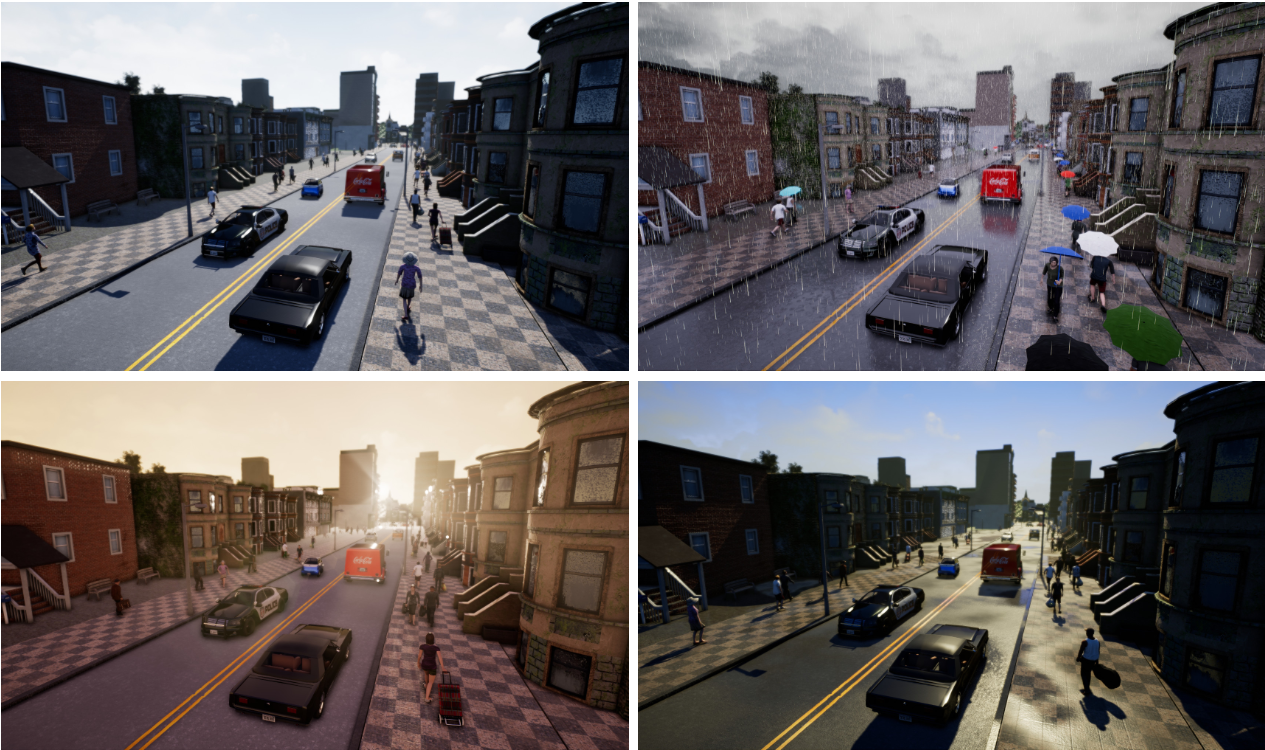
\includegraphics[width=0.9\textwidth]{img/carla_clima_example}
    \caption{Condiciones ambientales en el simulador CARLA.}
    \label{fig:carla-simulator}
\end{figure}

\subsection{Diseño del entorno de simulación}\label{subsec:simulation-design}

Para modelar el entorno de simulación, se propone un escenario de estacionamiento que incluye un vehículo y un espacio de estacionamiento.
La ubicación del vehículo, el espacio de estacionamiento y las condiciones ambientales se pueden inicializar de manera aleatoria en el simulador.
El vehículo estará equipado con sensores que proporcionarán los datos de entrada que se utilizarán para estimar la posición del vehículo con respecto al espacio de estacionamiento.
Estos sensores incluirán cámaras y sonar para capturar imágenes y distancias, respectivamente.

En la figura~\ref{fig:simulation-design} se muestra un ejemplo de cómo se podría diseñar el entorno de simulación.

\begin{figure}[!ht]
    \centering
    \begin{subfigure}{0.4\textwidth}
        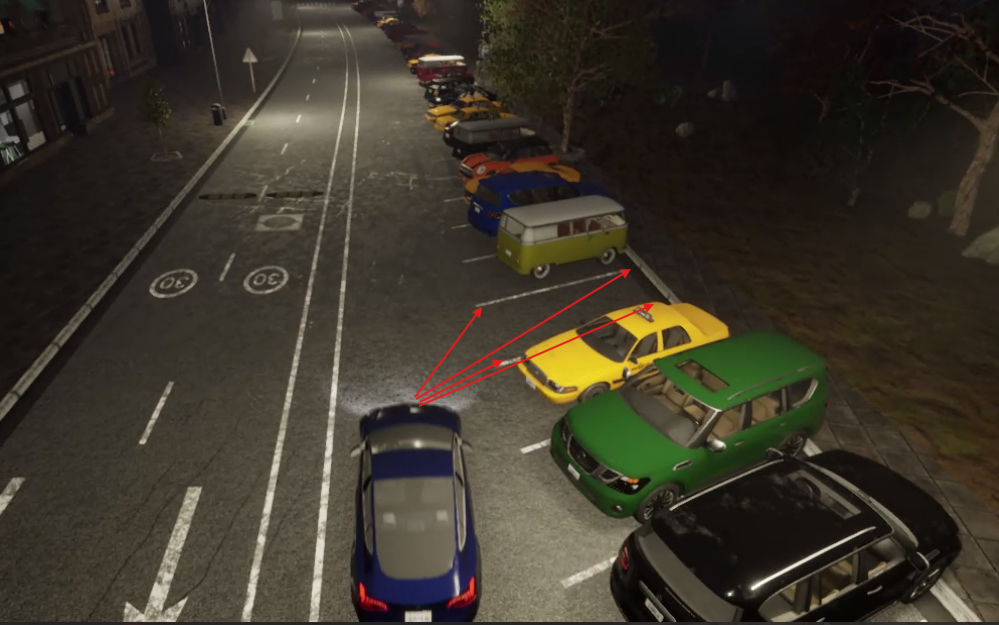
\includegraphics[width=\textwidth]{img/distances}\label {fig:distances}
    \end{subfigure}
    \begin{subfigure}{0.4\textwidth}
        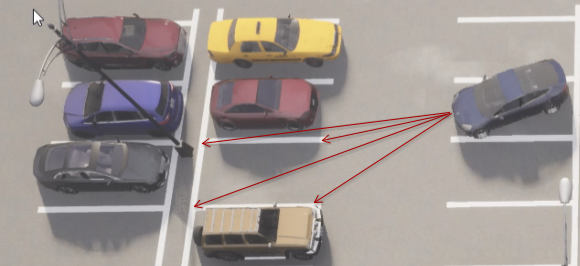
\includegraphics[width=\textwidth]{img/distances2}\label {fig:distances2}
    \end{subfigure}
    
    \caption{Diseño del entorno de simulación en CARLA.}
    \label{fig:simulation-design}
\end{figure}

\noindent
La cámara del vehículo capturará imágenes del entorno y el espacio de estacionamiento y el simulador permite ubicarla a conveniencia en el vehículo.

La ubicación de la cámara estará en la zona delantera del vehículo a una altura conocida (detrás del retrovisor). La siguiente figura ~\ref{fig:camera-view} muestra un ejemplo de como se visualiza el entorno desde la perspectiva de la cámara.

\begin{figure}[!ht]
    \centering
    \begin{subfigure}{0.4\textwidth}
        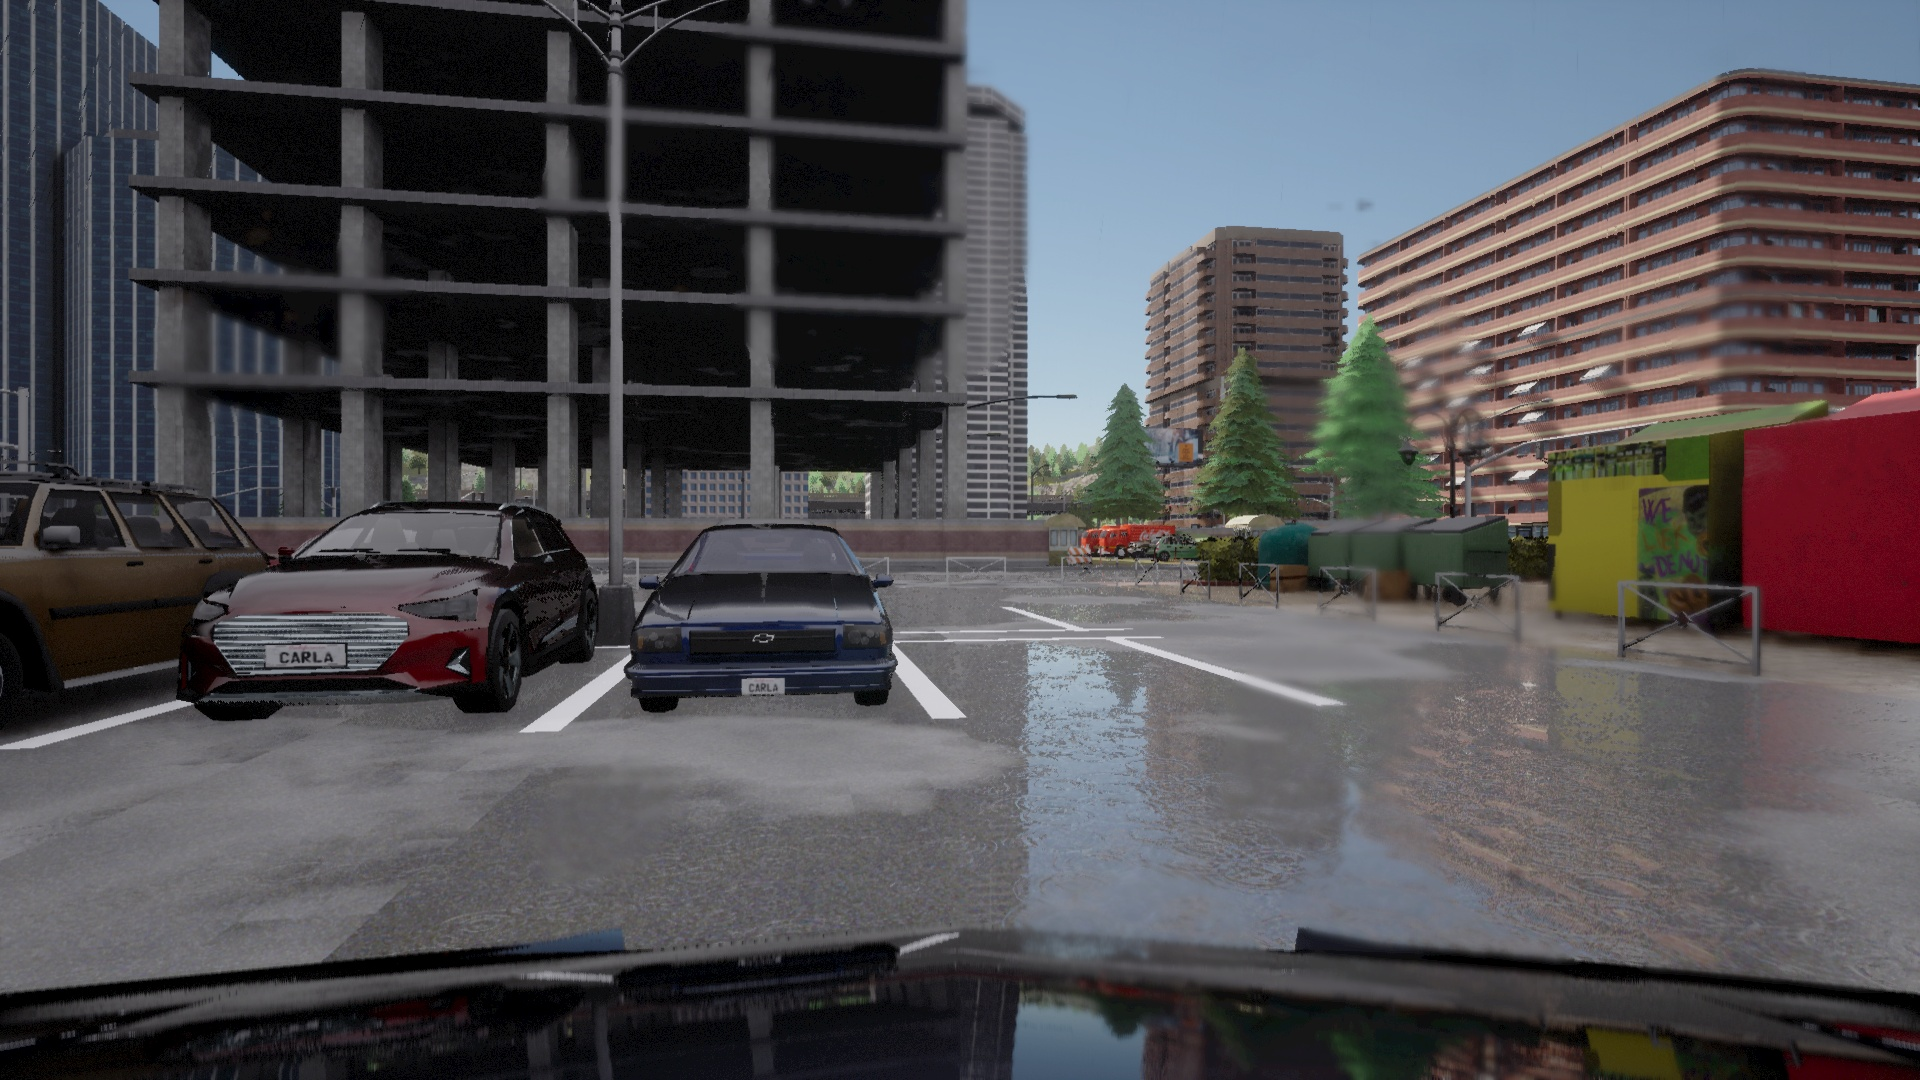
\includegraphics[width=\textwidth]{img/mirrow_camara_ex}\label {fig:camara}
    \end{subfigure}
    \begin{subfigure}{0.4\textwidth}
        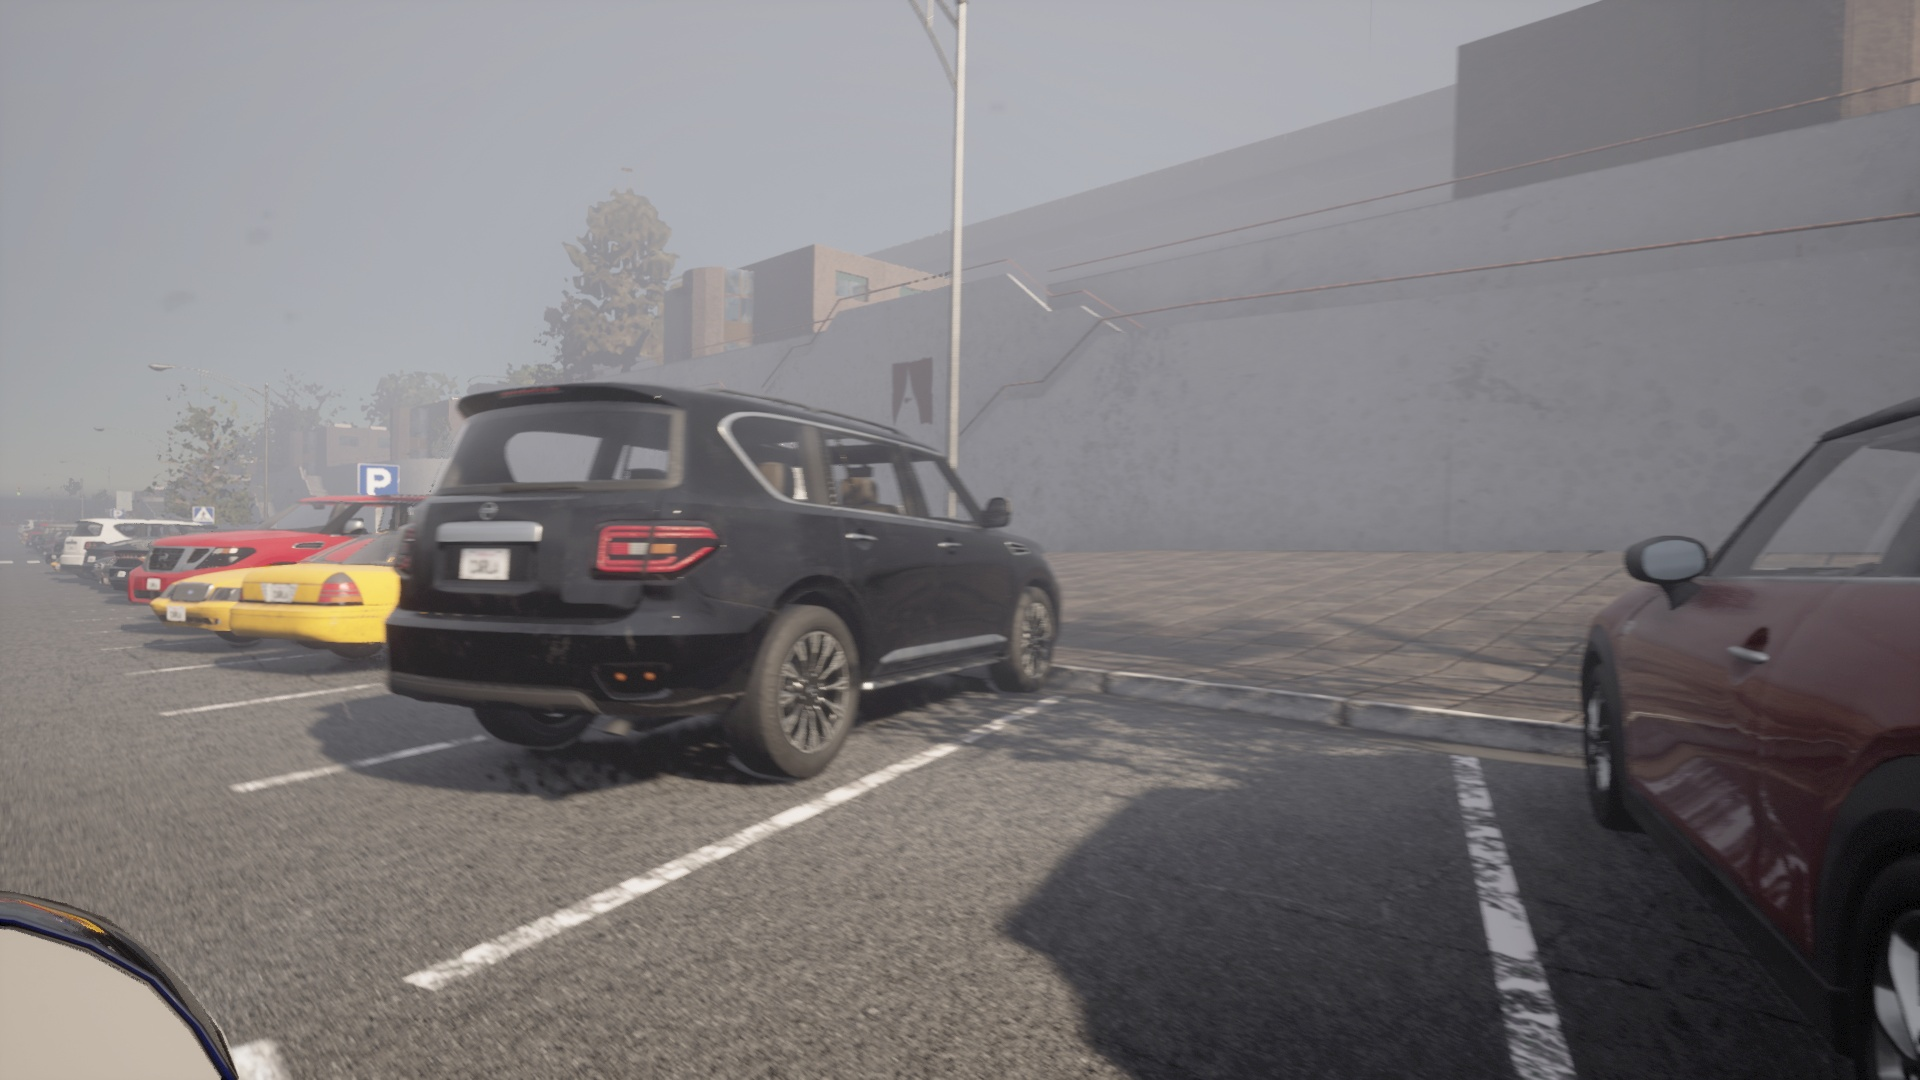
\includegraphics[width=\textwidth]{img/mirrow_camara_ex2}\label {fig:camara2}
    \end{subfigure}
    \caption{Vista de la cámara en el entorno de simulación.}
    \label{fig:camera-view}
\end{figure}





    \clearpage

    \section*{Detección de la retícula de estacionamiento}
    \noindent
Cuando proyectamos un escena del mundo real en tres dimensiones a un plano de dos dimensiones como la película o el sensor de una cámara, se produce una transformación en la imagen.
Esta transformación, que se conoce como transformación proyectiva, provoca que las líneas paralelas en el mundo real al proyectarse en el plano de la cámara se intersecten en un punto. A dicho punto se le conoce como punto de fuga.

\begin{figure}[!ht]
    \centering
    \begin{subfigure}{0.4\textwidth}
        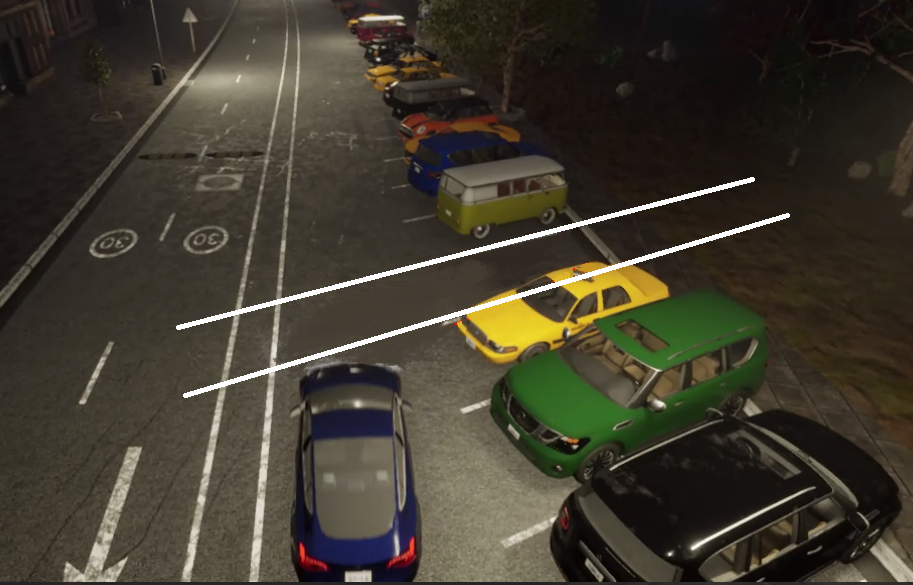
\includegraphics[width=\textwidth]{img/reticule/paralel_lines}\label {fig:parallel_lines}
        \caption{Ejemplo de líneas paralelas en un escenario real en 3 dimensiones}
    \end{subfigure}
    \begin{subfigure}{0.4\textwidth}
        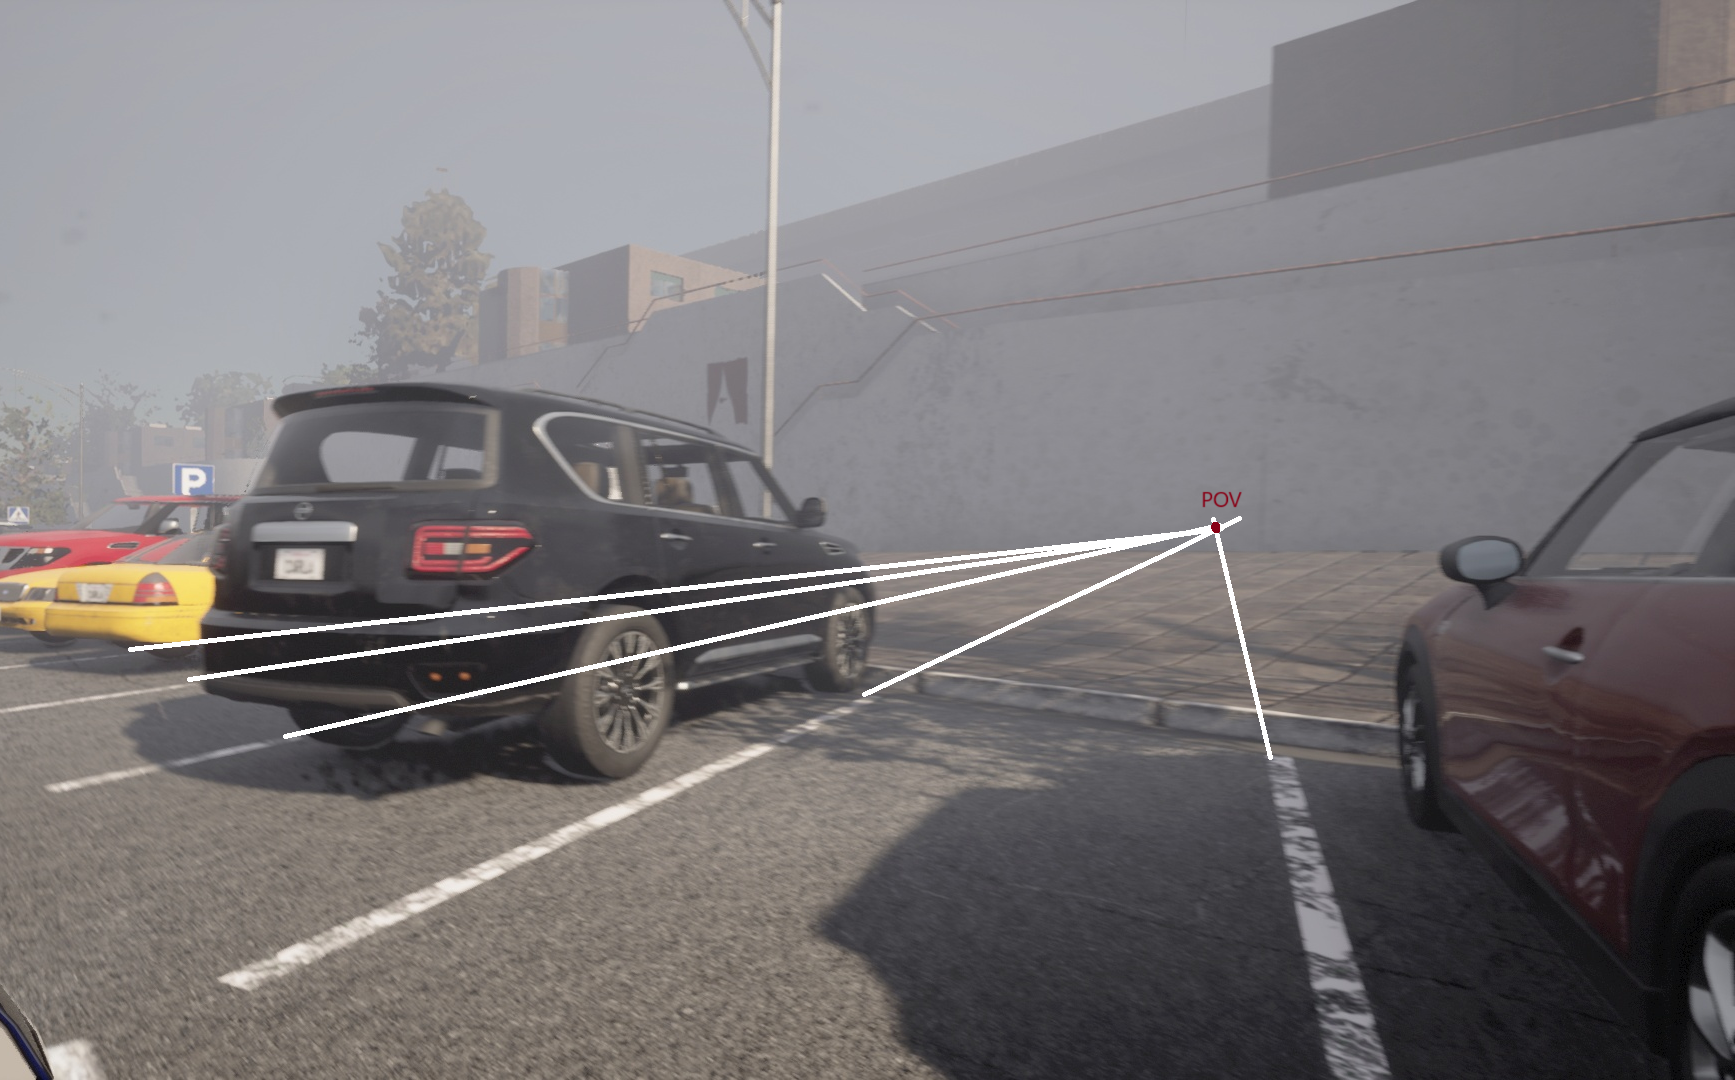
\includegraphics[width=\textwidth]{img/reticule/pov}\label {fig:pov}
        \caption{Proyección de líneas paralelas en el plano de la cámara}
    \end{subfigure}

    \label{fig:distorion}
\end{figure}

\noindent
Dado que las líneas de los cajones de estacionamiento son paralelas por su geometría, forman patrones en una retícula de paralelogramos.
Esto permite utilizar técnicas de detección de líneas para identificar los puntos de fuga y estimar la posición de la retícula de estacionamiento.

\begin{figure}[!ht]
    \centering
    \begin{subfigure}{0.8\textwidth}
        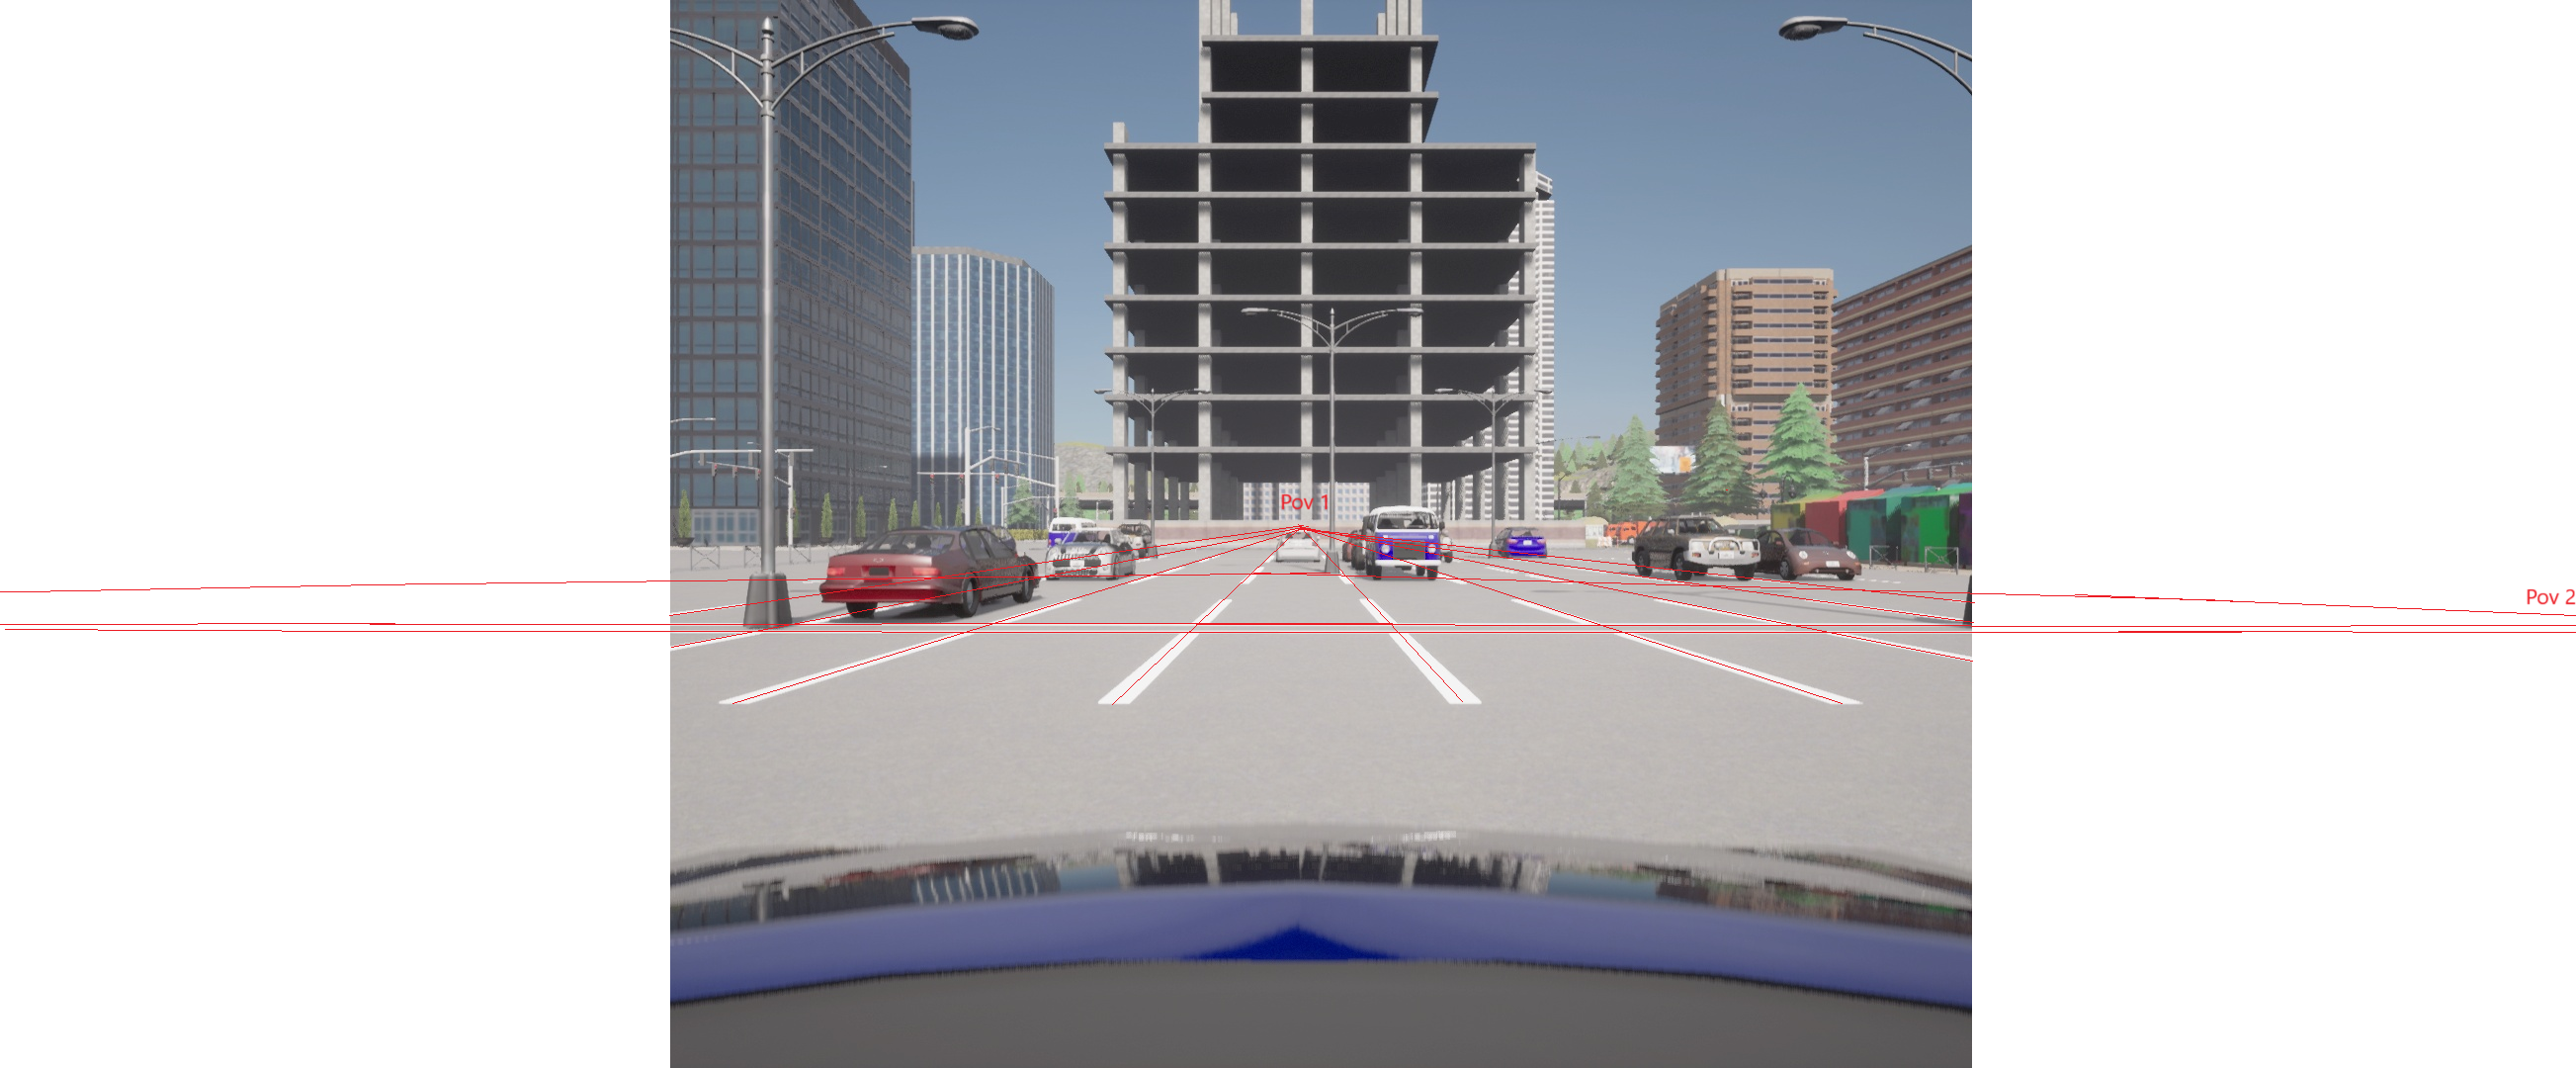
\includegraphics[width=\textwidth]{img/reticule/pov_reticule}\label {fig:pov_reticule}
    \end{subfigure}
    \begin{subfigure}{0.8\textwidth}
        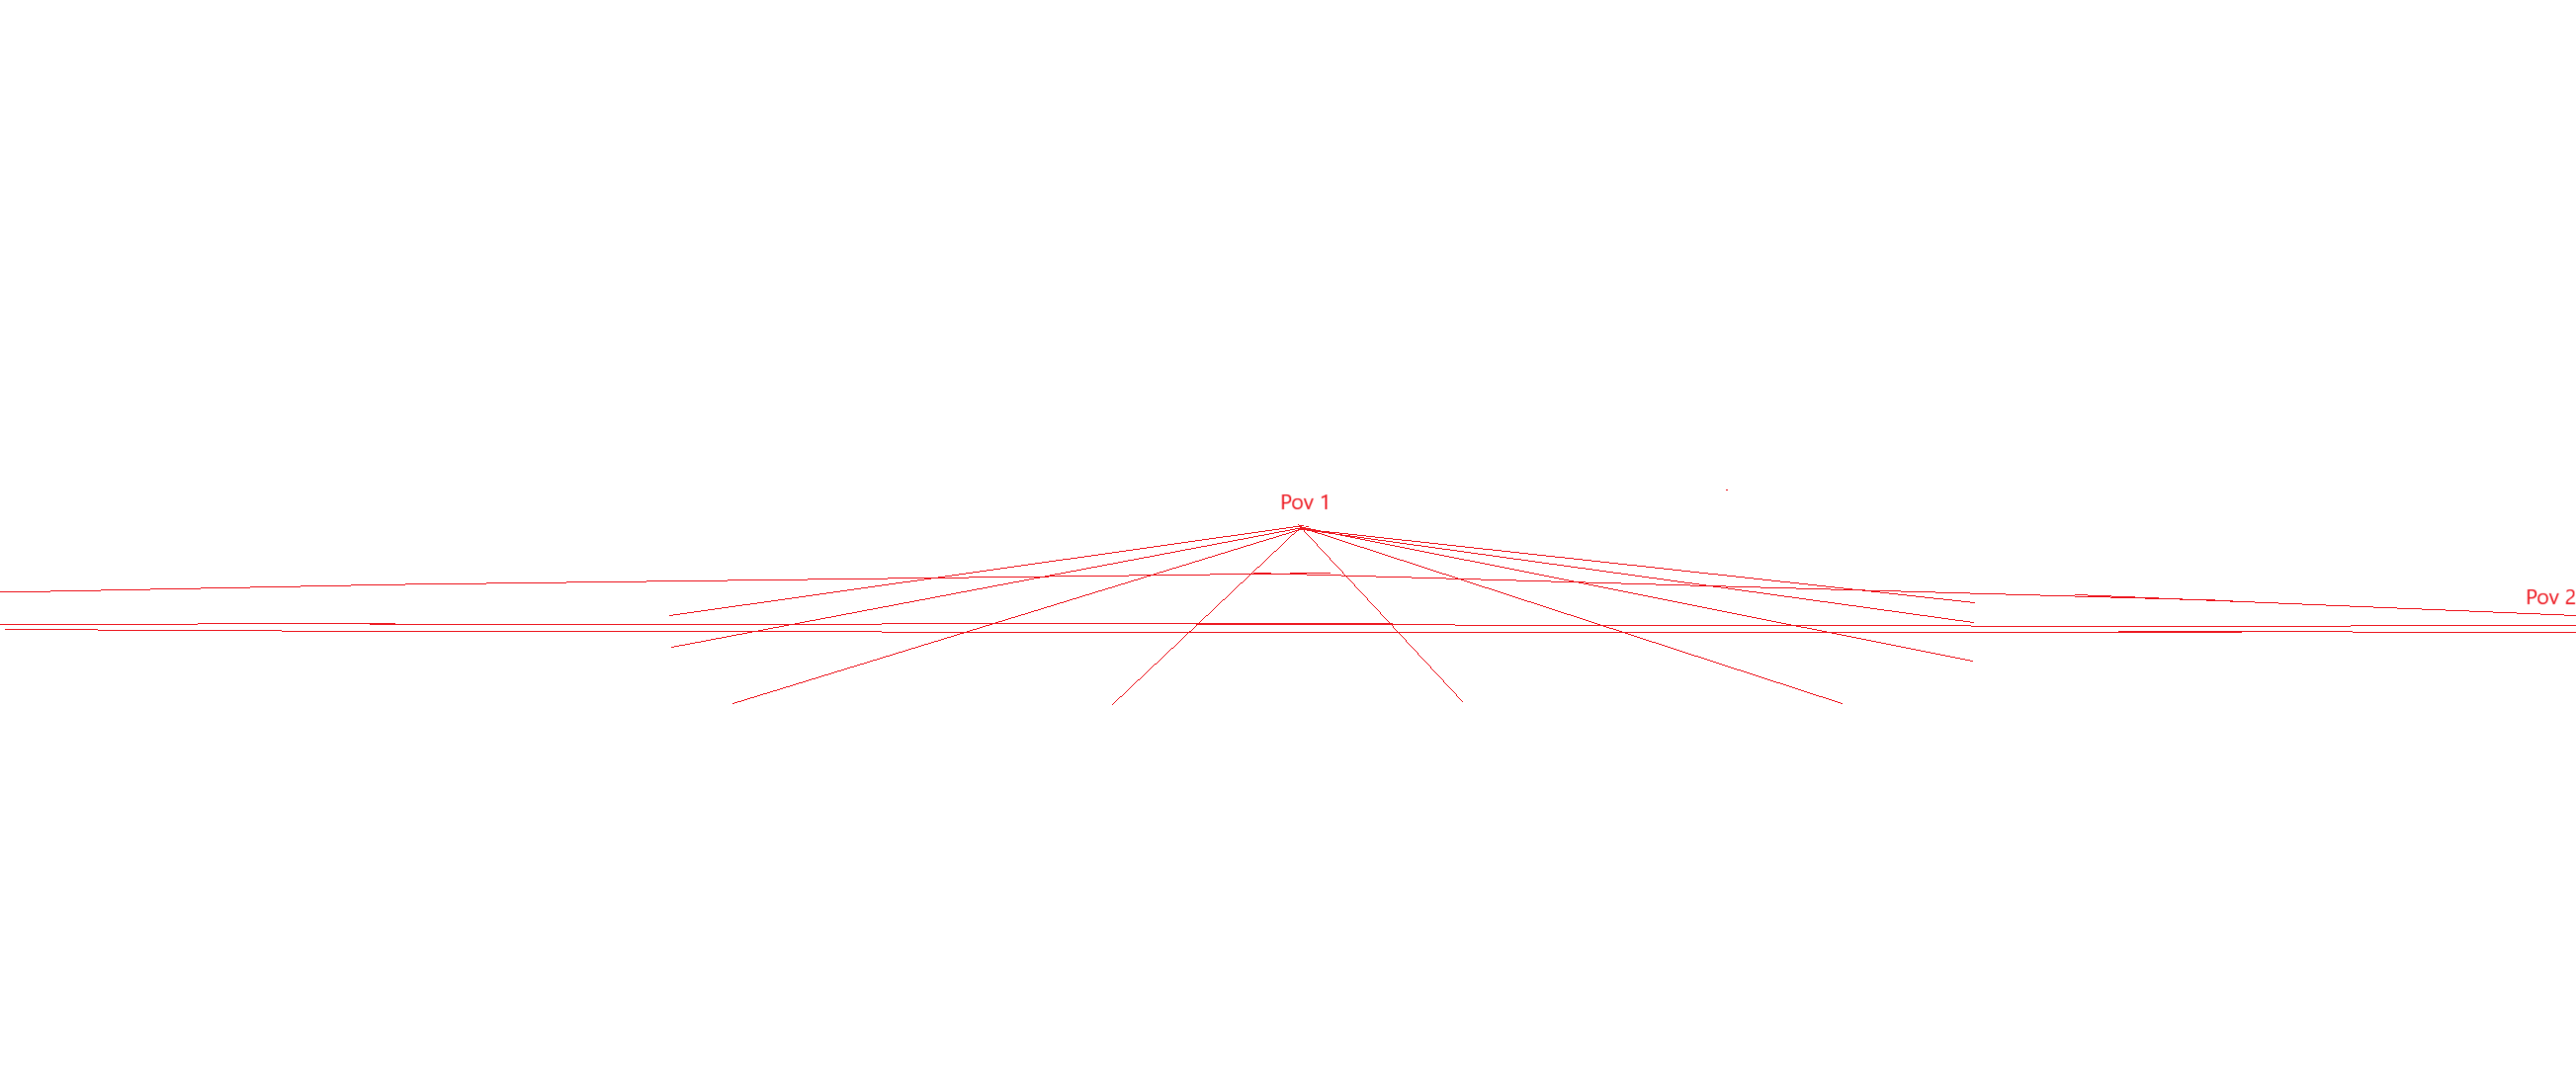
\includegraphics[width=\textwidth]{img/reticule/pov_reticule_layer}\label {fig:pov_reticule_layers}
    \end{subfigure}
    \caption{Líneas paralelas de la retícula de estacionamiento}
    \label{fig:reticule_pov}
\end{figure}

\noindent

\subsection{Detección de líneas paralelas:}

\begin{itemize}
    \item Área de interés:

    Teniendo en cuenta que la camara del vehículo se encuentra ubicada en la parte delantera a una altura conocida y en un ángulo paralelo al suelo, el área de interés de la imagen donde se encuentran las líneas de los cajones de estacionamiento quedara siempre por debajo del horizonte de la imagen.
    Por lo tanto, se puede eliminar la parte superior de la imagen para
    reducir el ruido y mejorar la detección de las líneas.
    \begin{figure}[!ht]
        \centering
        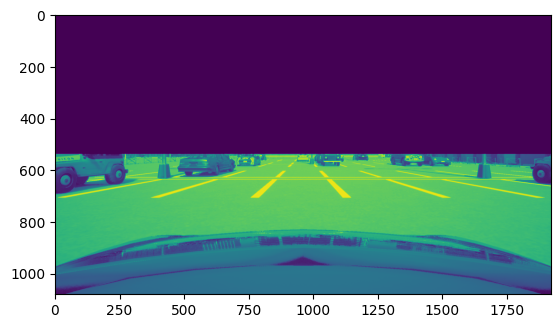
\includegraphics[width=0.6\textwidth]{img/reticule/horizont}
        \caption{Área de interés de la imagen}
        \label{fig:roi}
    \end{figure}

    \item Umbralización:

    Al área de interés de la imagen se le aplica una umbralización para realzar las líneas blancas de los cajones de estacionamiento y eliminar otros elementos no relevantes que puedan interferir en la detección.
    \begin{figure}[!ht]
        \centering
        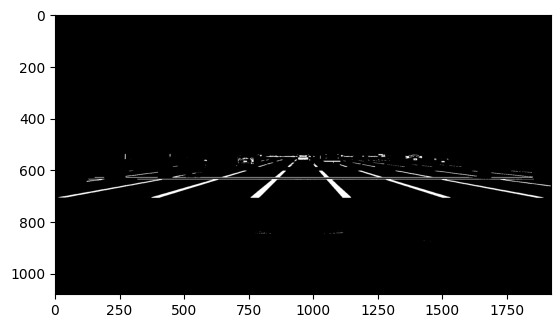
\includegraphics[width=0.6\textwidth]{img/reticule/thresholded}
        \caption{Imagen umbralizada}
        \label{fig:threshold}
    \end{figure}

    \clearpage
    \item Detección de contornos:

    Se utiliza el algoritmo de Canny para detectar los bordes de las líneas en la imagen umbralizada.
    \begin{figure}[!ht]
        \centering
        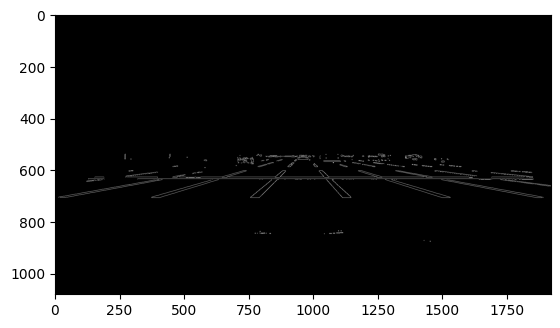
\includegraphics[width=0.6  \textwidth]{img/reticule/canny}
        \caption{Detección de bordes mediante el algoritmo de Canny}
        \label{fig:edges}
    \end{figure}

    \item Detección de líneas:

    Se aplica la transformada de Hough para detectar las coordenadas de inicio y fin de las líneas en la imagen.
    \begin{figure}[!ht]
        \begin{subfigure}{0.5\textwidth}
            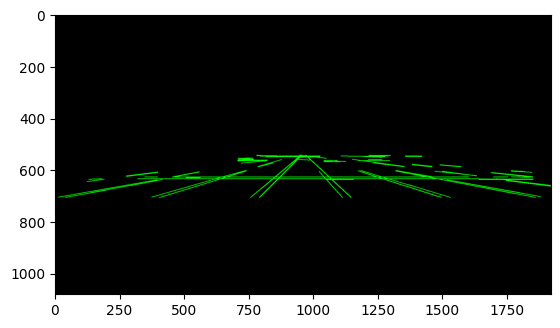
\includegraphics[width=\textwidth]{img/reticule/hough2}
            \caption{Líneas detectadas con la transformada de Hough}
            \label{fig:hough}
        \end{subfigure}
        \begin{subfigure}{0.5\textwidth}
            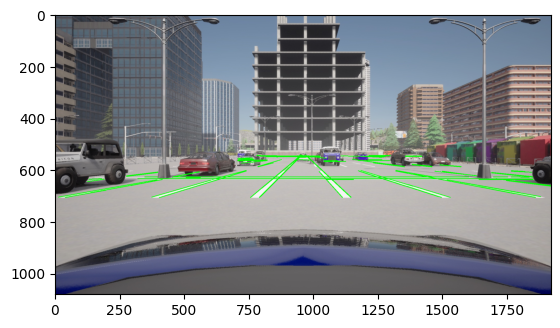
\includegraphics[width=\textwidth]{img/reticule/hough}
            \caption{Líneas detectadas en la imagen original}
            \label{fig:lines}
        \end{subfigure}
    \end{figure}

    \item Representación de las ecuaciones de las líneas:

    Una vez obtenidas las coordenadas de inicio y fin de cada línea paralela, podemos utilizar la ecuación general de la recta:
    \begin{equation}
        Ax + By + C = 0
    \end{equation}
    Esta ecuación nos permite determinar la orientación de cada línea.
    Dado que las coordenadas iniciales y finales de cada línea corresponden a los valores de $x$ y $y$, respectivamente,    estas se pueden emplear para formular un sistema de ecuaciones que describa los parámetros de la recta $[A, B, C]$.
    Dicho sistema puede representarse de manera matricial como sigue:
    \begin{equation}
        \begin{aligned}
            \left[\begin{array}{ccc}
                      x_1 & y_1 & 1 \\
                      x_2 & y_2 & 1
            \end{array}\right]
            \begin{bmatrix}
                A \\
                B \\
                C
            \end{bmatrix}
            =
            \begin{bmatrix}
                0 \\
                0
            \end{bmatrix}
        \end{aligned}
    \end{equation}

    Esta representación permite calcular de forma precisa los coeficientes de la ecuación de la recta para cada línea detectada, lo que es fundamental para analizar su orientación y posición dentro de la retícula de estacionamiento.

    \item Cálculo de ecuaciones de las líneas:

    Para calcular los coeficientes $[A, B, C]$ de las ecuaciones de las líneas detectadas, se utiliza el concepto de espacio nulo (\emph{null space}). Este enfoque se basa en el hecho de que cualquier vector en el espacio nulo de una matriz $\mathbf{M}$ satisface la ecuación
    \begin{equation}
        \mathbf{Mv} = 0
    \end{equation}

%Comentario: No has definido el vector v.


    Cada línea se representa mediante dos puntos $(x_1, y_1)$ y $(x_2, y_2)$. A partir de estas coordenadas homogeneas, construimos una matriz $\mathbf{M}$ de la forma:
    \[
        \mathbf{M} = \begin{bmatrix}
                         x_1 & y_1 & 1 \\
                         x_2 & y_2 & 1
        \end{bmatrix}
    \]
    Esta matriz define el sistema de ecuaciones que describe la recta que pasa por los puntos dados.
    El espacio nulo de $\mathbf{M}$ corresponde al conjunto de vectores $[A,B,C]$ que satisfacen
    \[
        \mathbf{M} \cdot \begin{bmatrix}
                             A \\ B \\ C
        \end{bmatrix} = \mathbf{0}.
    \]
    Se utiliza la Descomposición en Valores Singulares (SVD) para calcular este espacio nulo, ya que es una herramienta robusta y numéricamente estable.
    La SVD descompone la matriz \(M\) en tres matrices \(U\), \(S\) y \(V\), donde el espacio nulo de \(M\) se puede obtener a partir de la última columna de la matriz \(V\), que corresponde al vector singular más pequeño (el más cercano al cero).
    El vector resultante del espacio nulo se normaliza para que tenga una magnitud manejable.
    Esto asegura que los coeficientes \(A\), \(B\) y \(C\) sean comparables entre distintas líneas.

    \item Cálculo de intersecciones:

    Dado que ya se tendrían las ecuaciones de todas las líneas paralelas en el plano de la cámara, se pueden calcular las intersecciones de estas líneas realizando un producto cruz entre las ecuaciones homogéneas [\(A\),\(B\),\(C\)] de todos los pares de líneas.

    El resultado de este producto cruz es la coordenada homogénea de un punto en el espacio que corresponde a la intersección de las líneas.
    Si este punto es finito (cuando la tercera componente no es cero), se puede deshomogenizar para obtener las coordenadas cartesianas en el plano de la cámara.
    En cambio, si el punto es infinito (cuando la tercera componente muy cercana a cero), significa que las líneas son paralelas y se intersectan en el infinito.


    \item  Agrupación de intersecciones:
    %https://scikit-learn.org/stable/modules/clustering.html#hierarchical-clustering

    Analizando los puntos de intersecciones obtenidos que se encuentran en el plano de la cámara, se pueden agrupar para determinar donde están
    concentrada la mayor cantidad de intersecciones.
    Este punto de concentración de intersecciones debe corresponder al punto de fuga principal de la retícula de estacionamiento.\\
    
    \begin{figure}[!ht]
        \centering
        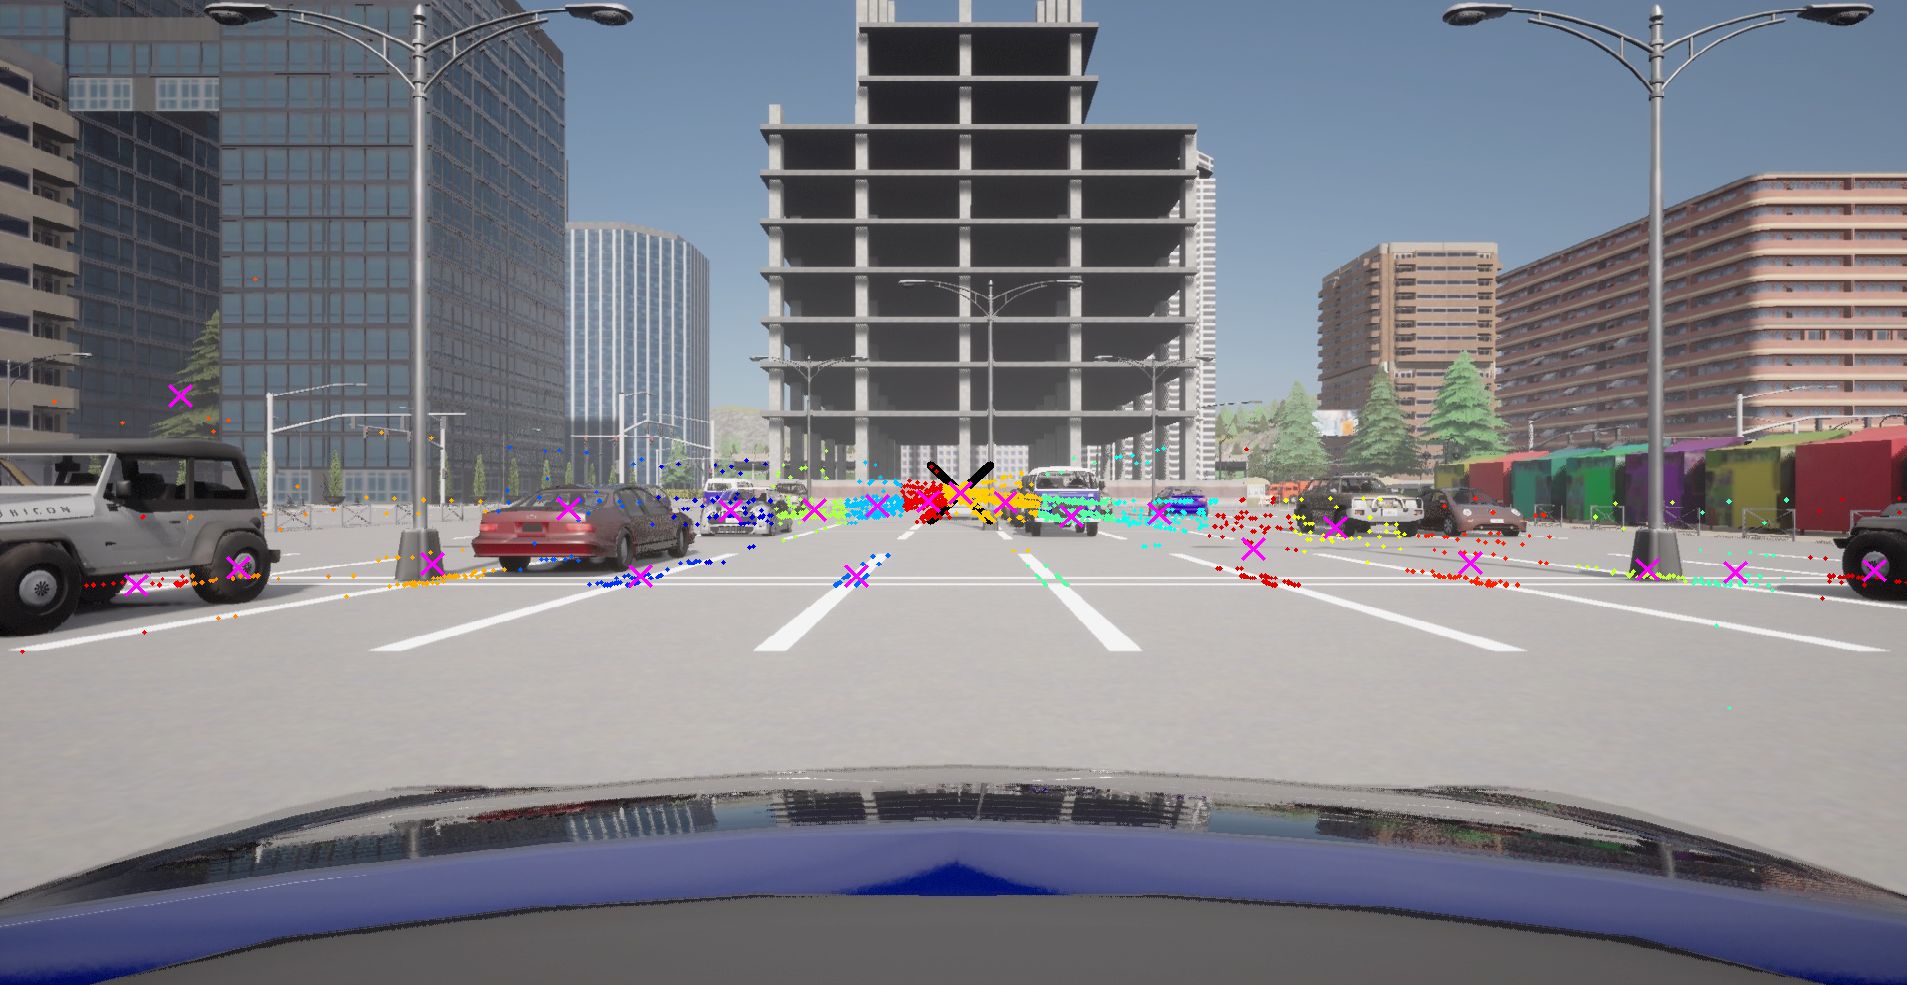
\includegraphics[width=0.8\textwidth]{img/reticule/svd-km}
        \caption{Agrupacion de intersecciones de las líneas detectadas}
        \label{fig:intersections}
    \end{figure}
    
    Para estimar la ubicación de este punto de fuga principal no es necesario tener en cuenta todas las intersecciones detectadas,
    sino solo aquellas que se encuentran en una zona cercana al horizonte de la imagen.
    Esto se debe a que, debido a la perspectiva de la cámara, las líneas paralelas en el mundo real convergen hacia el horizonte en la imagen,
    haciendo que los puntos de fuga se ubiquen cerca de esta línea.
    Para determinar las intercepciones relevantes cercanas al horizonte, se puede definir un umbral de cercanía en la imagen que se puede ajustar experimentalmente.
    Por ejemplo, en la siguiente imagen se muestran las intersecciones detectadas en la imagen original con puntos azules
    y las intersecciones relevantes con un umbral de 10 píxeles con puntos amarillos.
    \begin{figure}[!ht]
        \centering
        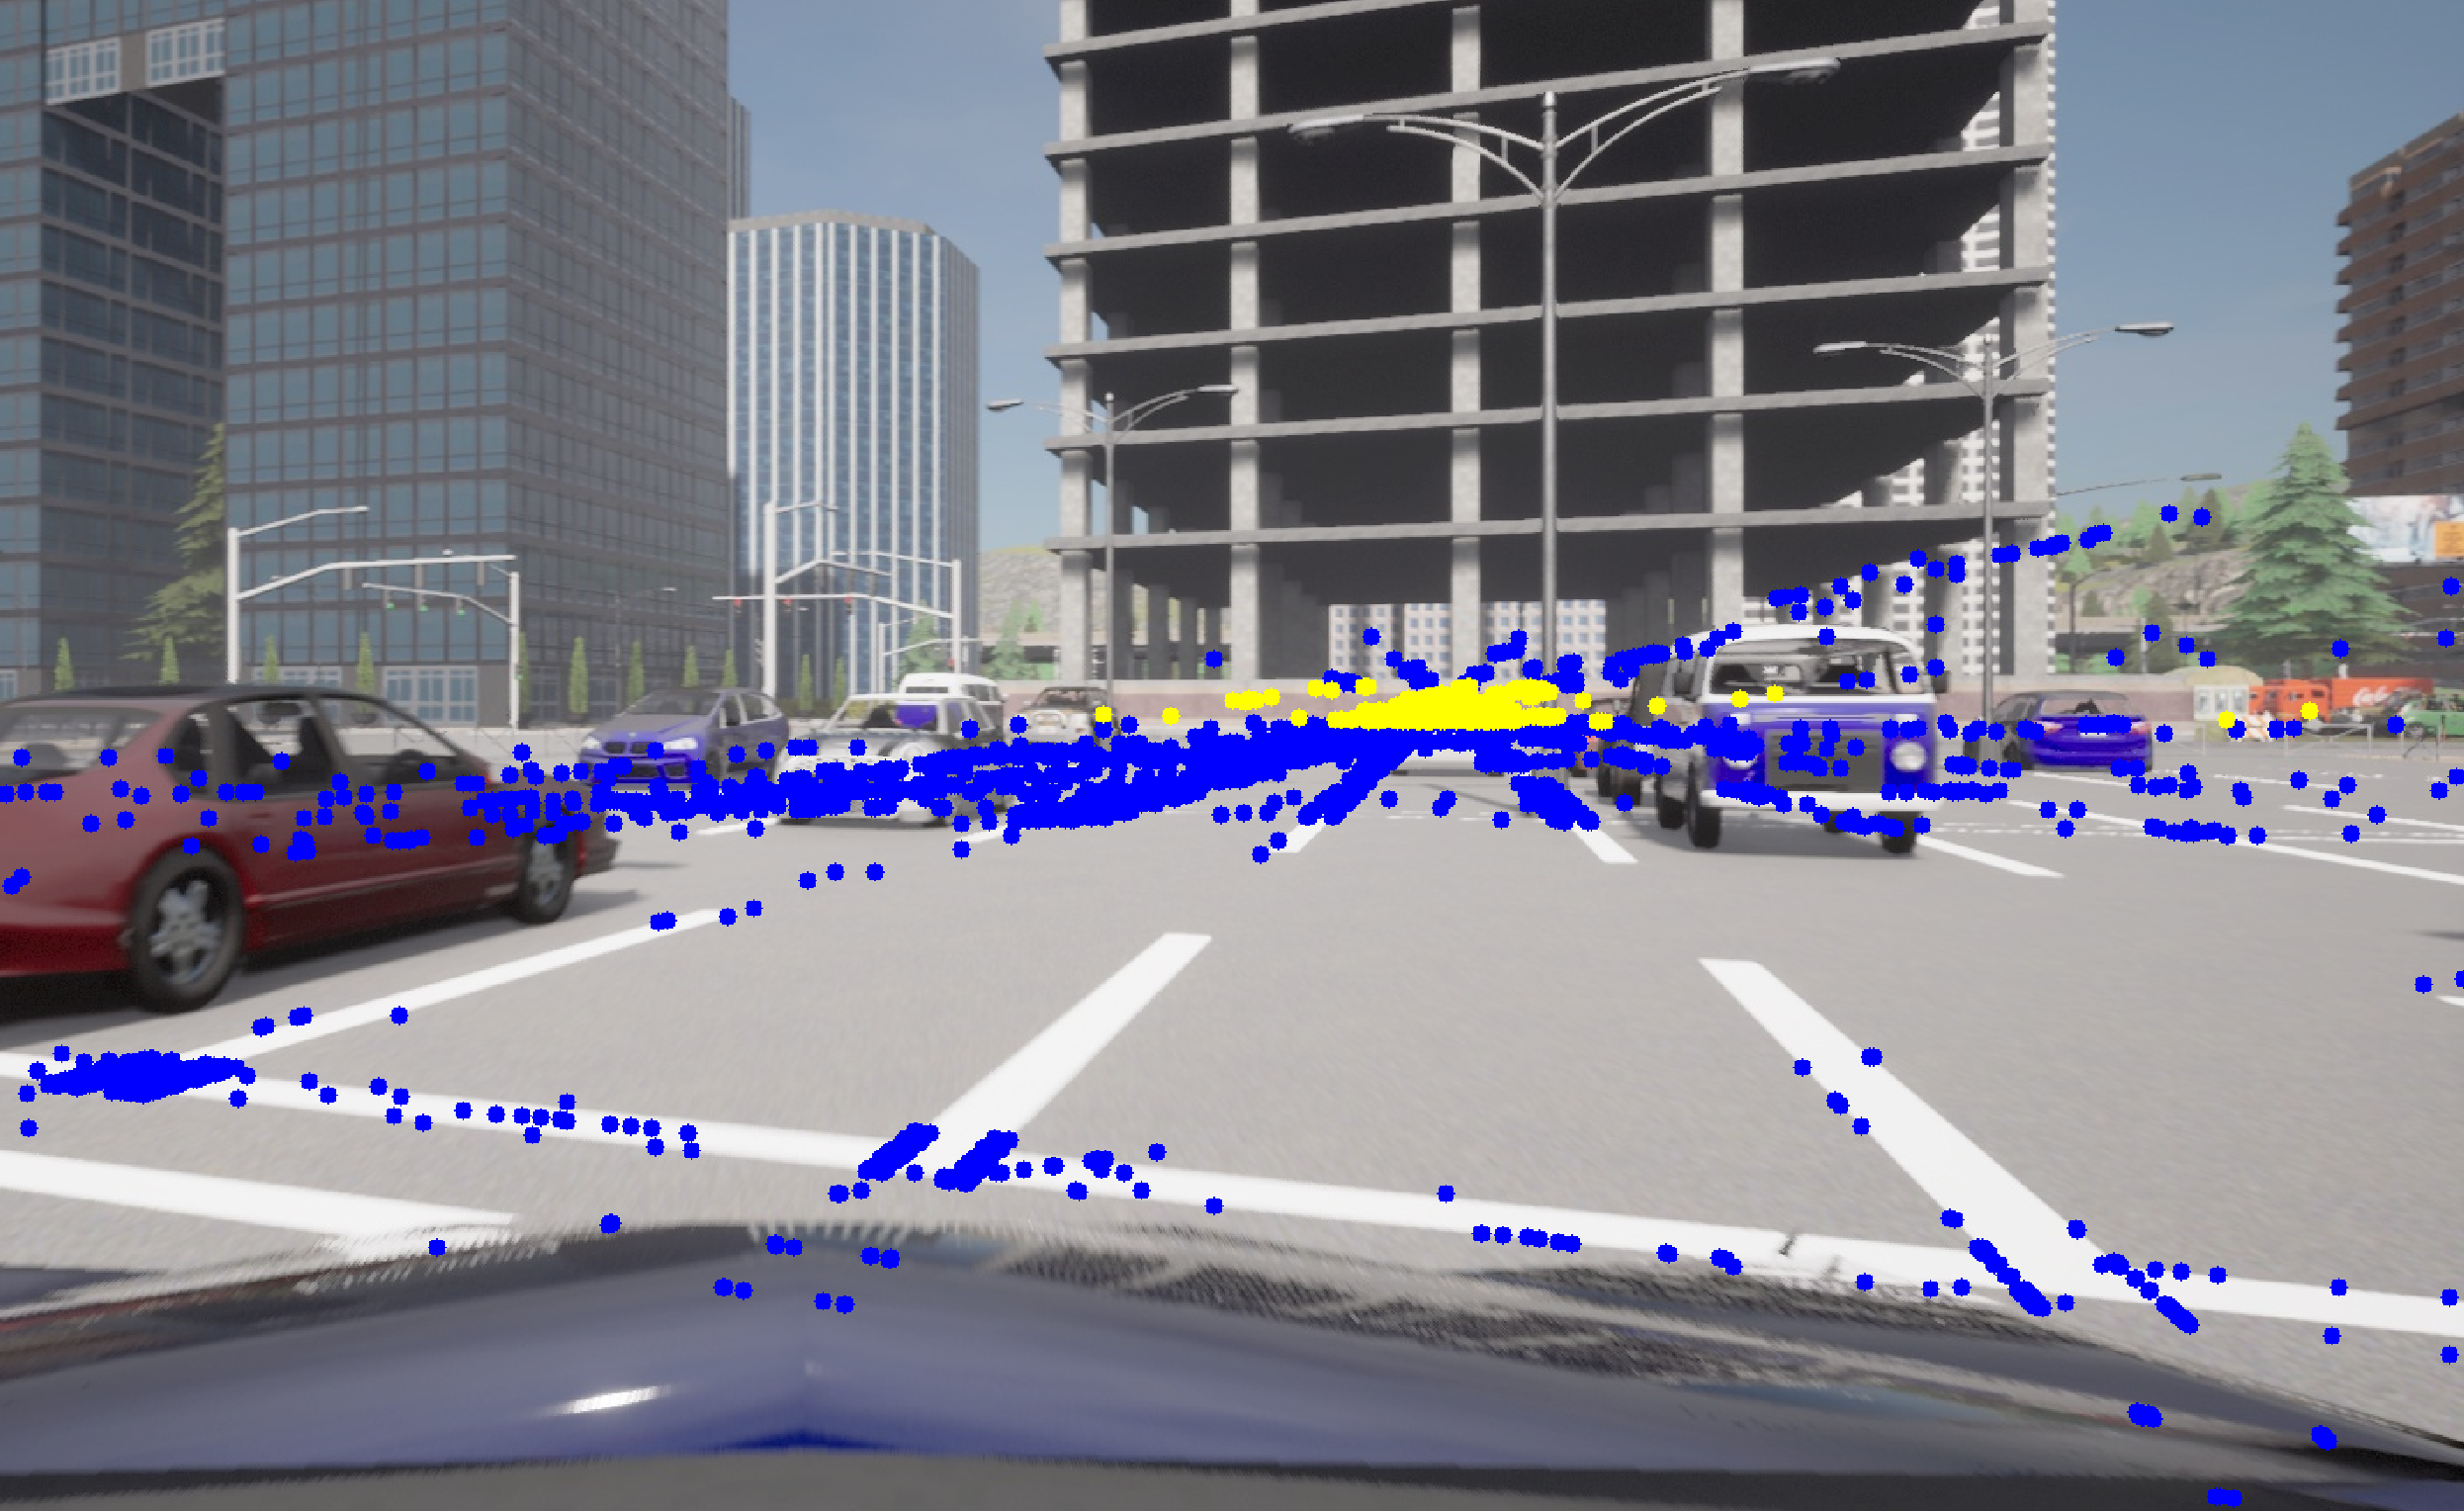
\includegraphics[width=0.8\textwidth]{img/reticule/relevantInter}
        \caption{Intersecciones detectadas en la imagen original}
        \label{fig:relevantInter}
    \end{figure}

    \item Algoritmo de agrupación:\\

    Para realizar la agrupación de las intersecciones relevantes, se utilizó el algoritmo \texttt{AgglomerativeClustering} de la librería \texttt{scikit-learn}.
    Este algoritmo fue elegido debido a su capacidad para manejar datos jerárquicos y su flexibilidad para determinar el número óptimo de clusters. Además,
    es robusto frente a la variabilidad en la densidad de los puntos de intersección.
    El algoritmo de agrupación jerárquica se basa en la idea de que los puntos cercanos entre sí pertenecen al mismo cluster.
    Para que el algoritmo determine el número de clusters se utilizo el parámetro \texttt{distance\_threshold} que indica la distancia máxima
    entre dos puntos para que se consideren en el mismo cluster. El valor de este parámetro se puede ajustar experimentalmente.
    Por ejemplo, en la siguiente imagen se muestran los mismos puntos de intersección relevantes del ejemplo anterior,
    pero agrupados por el algoritmo de agrupación jerárquica en 3 clusters representados de distintos colores con un símbolo \texttt{+} blanco en el centro de cada cluster.
    \begin{figure}[!ht]
        \centering
        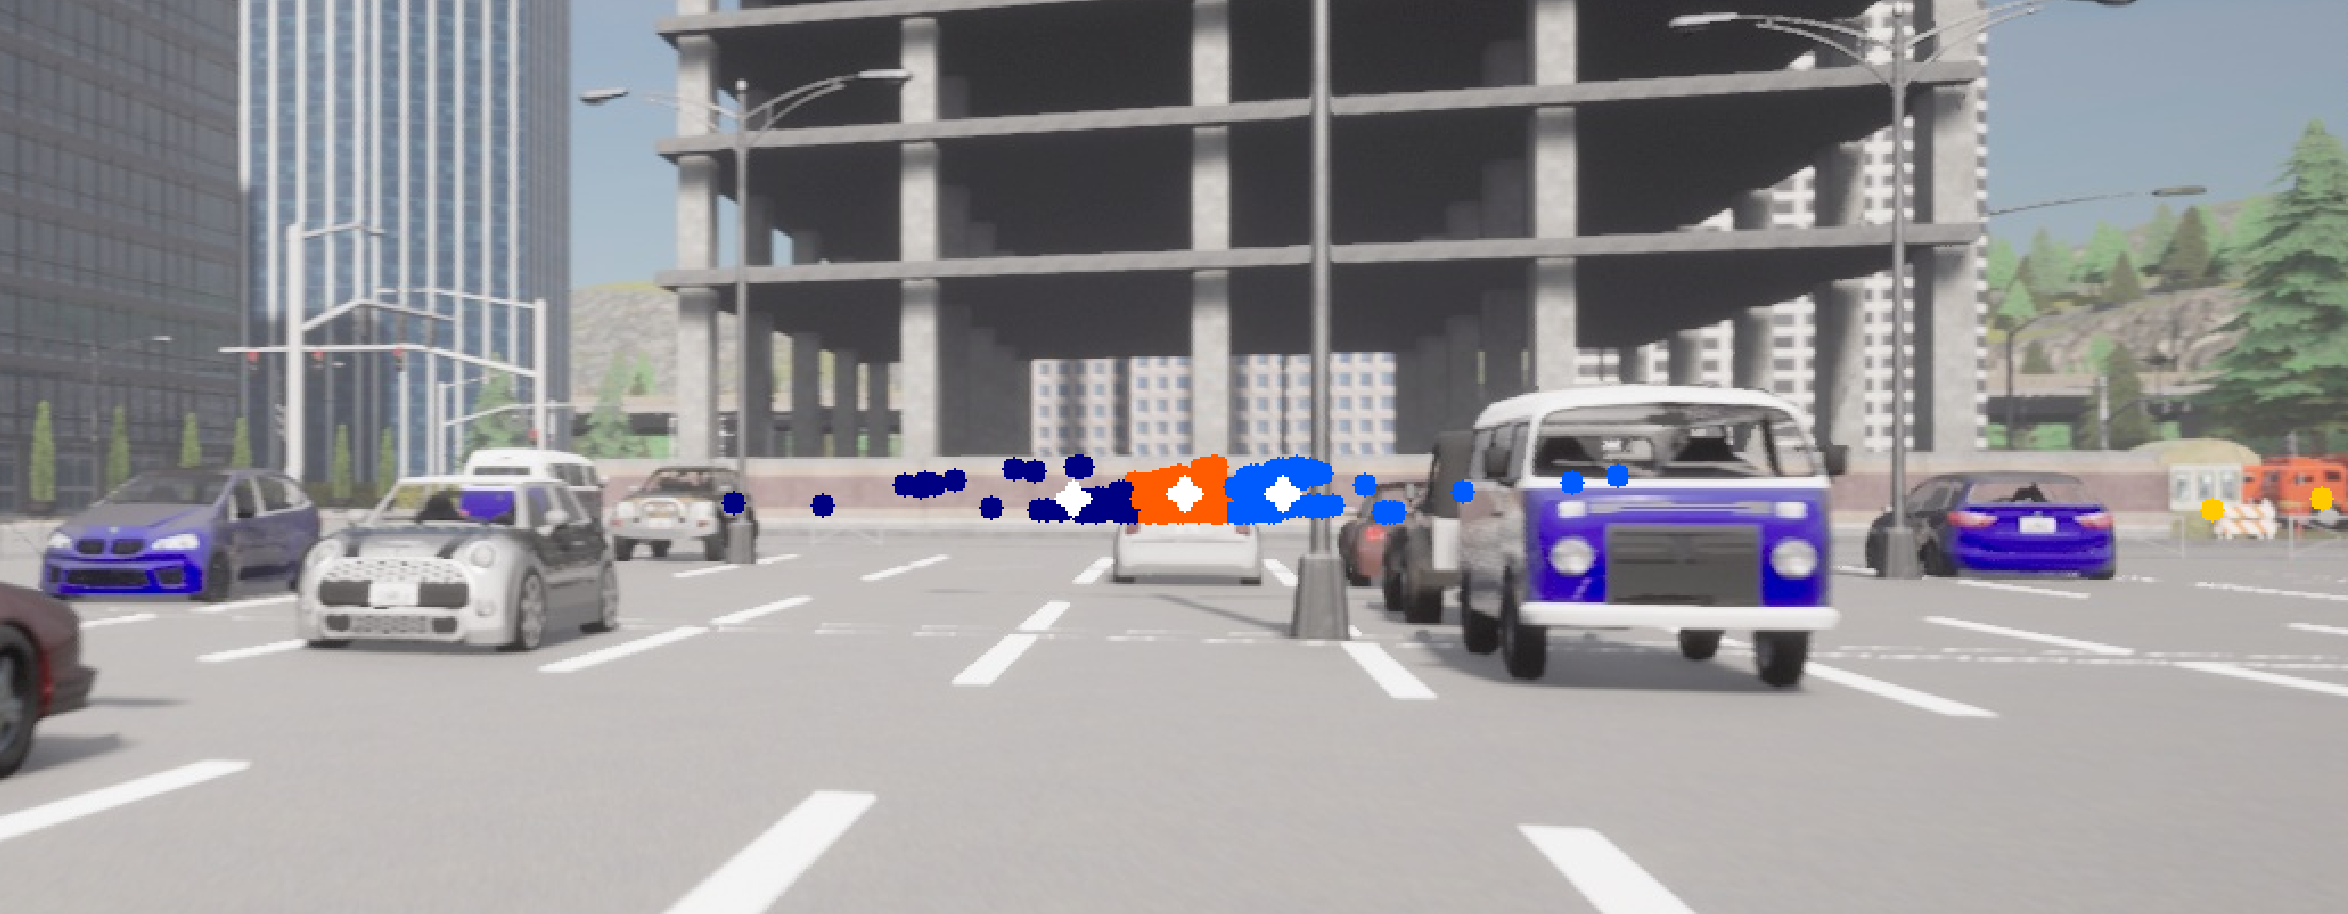
\includegraphics[width=0.8\textwidth]{img/reticule/AgglomerativeClustering}
        \caption{Intersecciones agrupadas en clusters}
        \label{fig:clusters}
    \end{figure}
    \item Selección del punto de fuga principal:\\
%    Intersección de n líneas
%    La intersección de n líneas (bajo un criterio de mínimos cuadrados) esta dado por
%    el eigen vector asociado al eigen valor más pequeño de la matriz $M$ donde:
%    $$
%    M = \sum_{i=1}^{n} w_i l_i l_i^T
%    $$
%    donde $w_i$ es un peso asociado a la linea $l_i$ y $l_i$ es la representación homogénea de la linea $i$.

%    Kanatani, K. (1998). Statistical optimization for geometric computation: theory and practice. Elsevier.
    Pata estimar la posición del punto de fuga principal, se puede seleccionar el cluster con mayor cantidad de intersecciones y
    utilizar las lineas que generaron estos puntos para calcular la intersección de estas lineas.
    La intersección de n líneas (bajo un criterio de mínimos cuadrados) esta dado por
    el eigen vector asociado al eigen valor más pequeño de la matriz $M$ donde:
    $$ M = \sum_{i=1}^{n} w_i l_i l_i^T $$
    donde $w_i$ es un peso asociado a la linea $l_i$ y $l_i$ es la representación homogénea de la linea $i$.
%    TODO: add ref
%    Kanatani, K. (1998). Statistical optimization for geometric computation: theory and practice. Elsevier.
    De esta forma podemos conocer la posición del punto de fuga principal en el plano de la cámara.
    en la siguiente imagen se muestra el resultado de esta estimacion utilizando las lineas del cluster más grande, donde se
    representa el punto de fuga principal con un símbolo \texttt{+} amarillo.
    \begin{figure}[!ht]
        \centering
        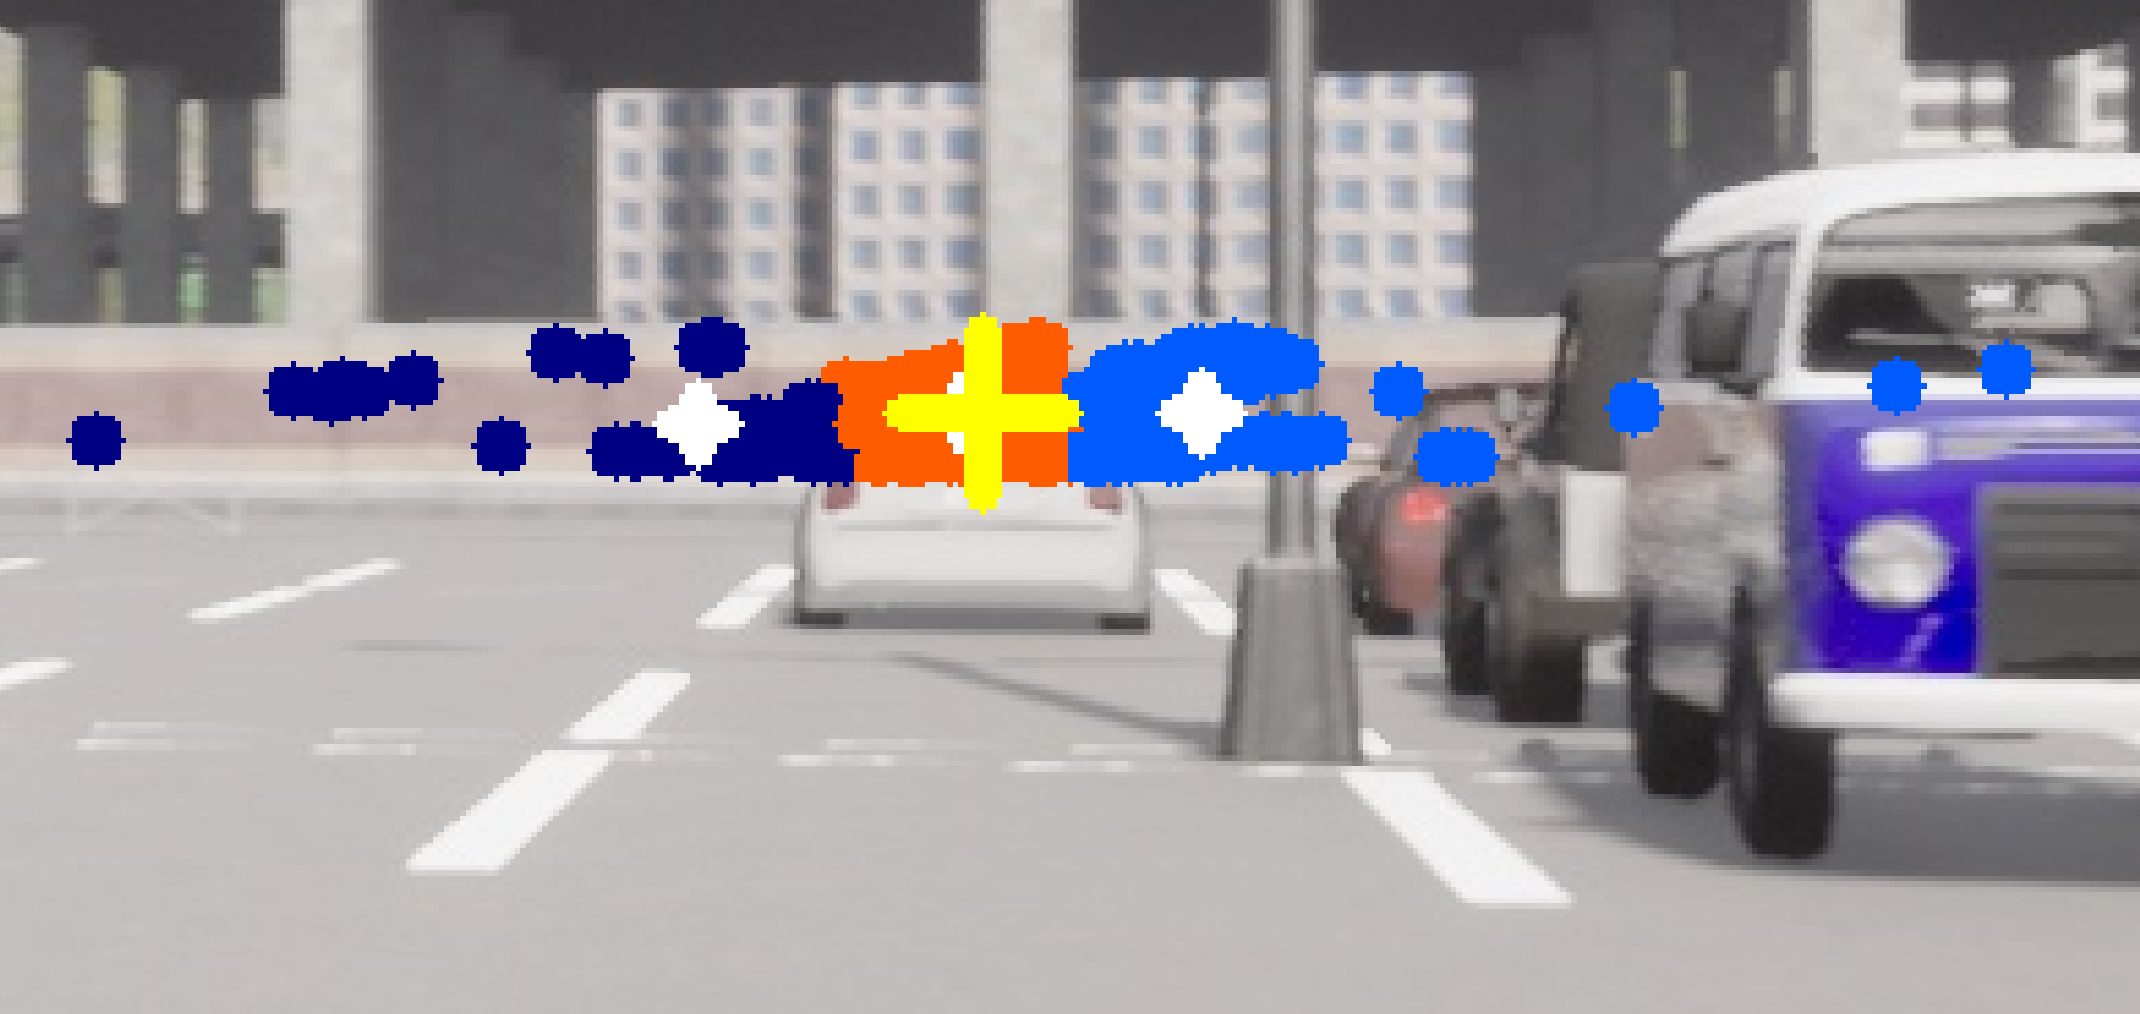
\includegraphics[width=0.8\textwidth]{img/reticule/vanishingPoint}
        \caption{Punto de fuga principal estimado}
        \label{fig:vanishingPoint}
    \end{figure}

    \item Selección del 2do punto de fuga principal:\\

    \item Estimación de la retícula de estacionamiento:


\end{itemize}

\subsection{Experimentación y ajuste de parámetros:}\label{subsec:experimentacion-y-ajuste-de-parametros:}
Para poder determinar la configuración conveniente de los parámetros que se utilizan en los distintos algoritmos que se usan en la solución propuesta,
se realizó una aplicación en Python carga una secuencia de imágenes de la trayectoria del vehículo en el estacionamiento y por cada frame,
calcula la retícula de estacionamiento aplicando los pasos anteriormente descritos.
La aplicación permite visualizar los resultados de cada paso y ajustar dinámicamente los parámetros de los algoritmos para obtener los mejores resultados.
Los parámetros ajustables que se consideraron son:
\begin{itemize}
    \item \texttt{threshold\_image}: Umbral de binarización de la imagen.
    \item \texttt{canny\_threshold\_1}: Umbral inferior para el algoritmo de Canny.
    \item \texttt{canny\_threshold\_2}: Umbral superior para el algoritmo de Canny.
    \item \texttt{hough\_rho}: Resolución de la distancia en píxeles de la cuadrícula de la transformada de Hough.
    \item \texttt{hough\_theta}: Resolución del ángulo en radianes de la cuadrícula de la transformada de Hough.
    \item \texttt{hough\_threshold}: Umbral de votación de la transformada de Hough.
    \item \texttt{hough\_min\_line\_length}: Longitud mínima de la línea en píxeles.
    \item \texttt{hough\_max\_line\_gap}: Máxima separación entre segmentos de línea para tratarlos como una sola línea.
    \item \texttt{relevant\_intersections\_horizon\_threshold}: Umbral de cercanía al horizonte para considerar una intersección relevante.
    \item \texttt{agglomerative\_distance\_threshold}: Distancia máxima entre dos puntos para considerarlos en el mismo cluster.
\end{itemize}
Para analizar el impacto del cambio en los parámetros en tiempo real, la aplicación provee un menu de acciones que permite
representar en la imagen los resultados de cada paso del algoritmo
%bloque de codigo
%\begin{lstlisting}[language=Python,label={lst:lstlisting22}]
%    --- Leyenda de Teclas ---
%P: Iniciar/Pausar la secuencia de imágenes.
%C: Mostrar/Ocultar contornos.
%L: Mostrar/Ocultar líneas.
%I: Mostrar/Ocultar intersecciones.
%R: Mostrar/Ocultar intersecciones relevantes.
%E: Mostrar/Ocultar líneas relevantes.
%A: Mostrar/Ocultar cúmulos de intersecciones.
%F: Mostrar/Ocultar puntos de fuga.
%G: Mostrar/Ocultar imagen binaria.
%ESC: Salir.
%\end{lstlisting}

\begin{verbatim}
    --- Leyenda de Teclas ---
P: Iniciar/Pausar la secuencia de imágenes.
C: Mostrar/Ocultar contornos.
L: Mostrar/Ocultar líneas.
I: Mostrar/Ocultar intersecciones.
R: Mostrar/Ocultar intersecciones relevantes.
E: Mostrar/Ocultar líneas relevantes.
A: Mostrar/Ocultar cúmulos de intersecciones.
F: Mostrar/Ocultar puntos de fuga.
G: Mostrar/Ocultar imagen binaria.
ESC: Salir.
\end{verbatim}

A continuación se muestra un ejemplo de la aplicación en ejecución en uno de los frames de la secuencia de imágenes,
donde se visualizan los contornos, las líneas detectadas, las intersecciones, las intersecciones relevantes, las líneas relevantes,
los cúmulos de intersecciones y los puntos de fuga.

\begin{figure}[!ht]
    \begin{subfigure}{0.5\textwidth}
        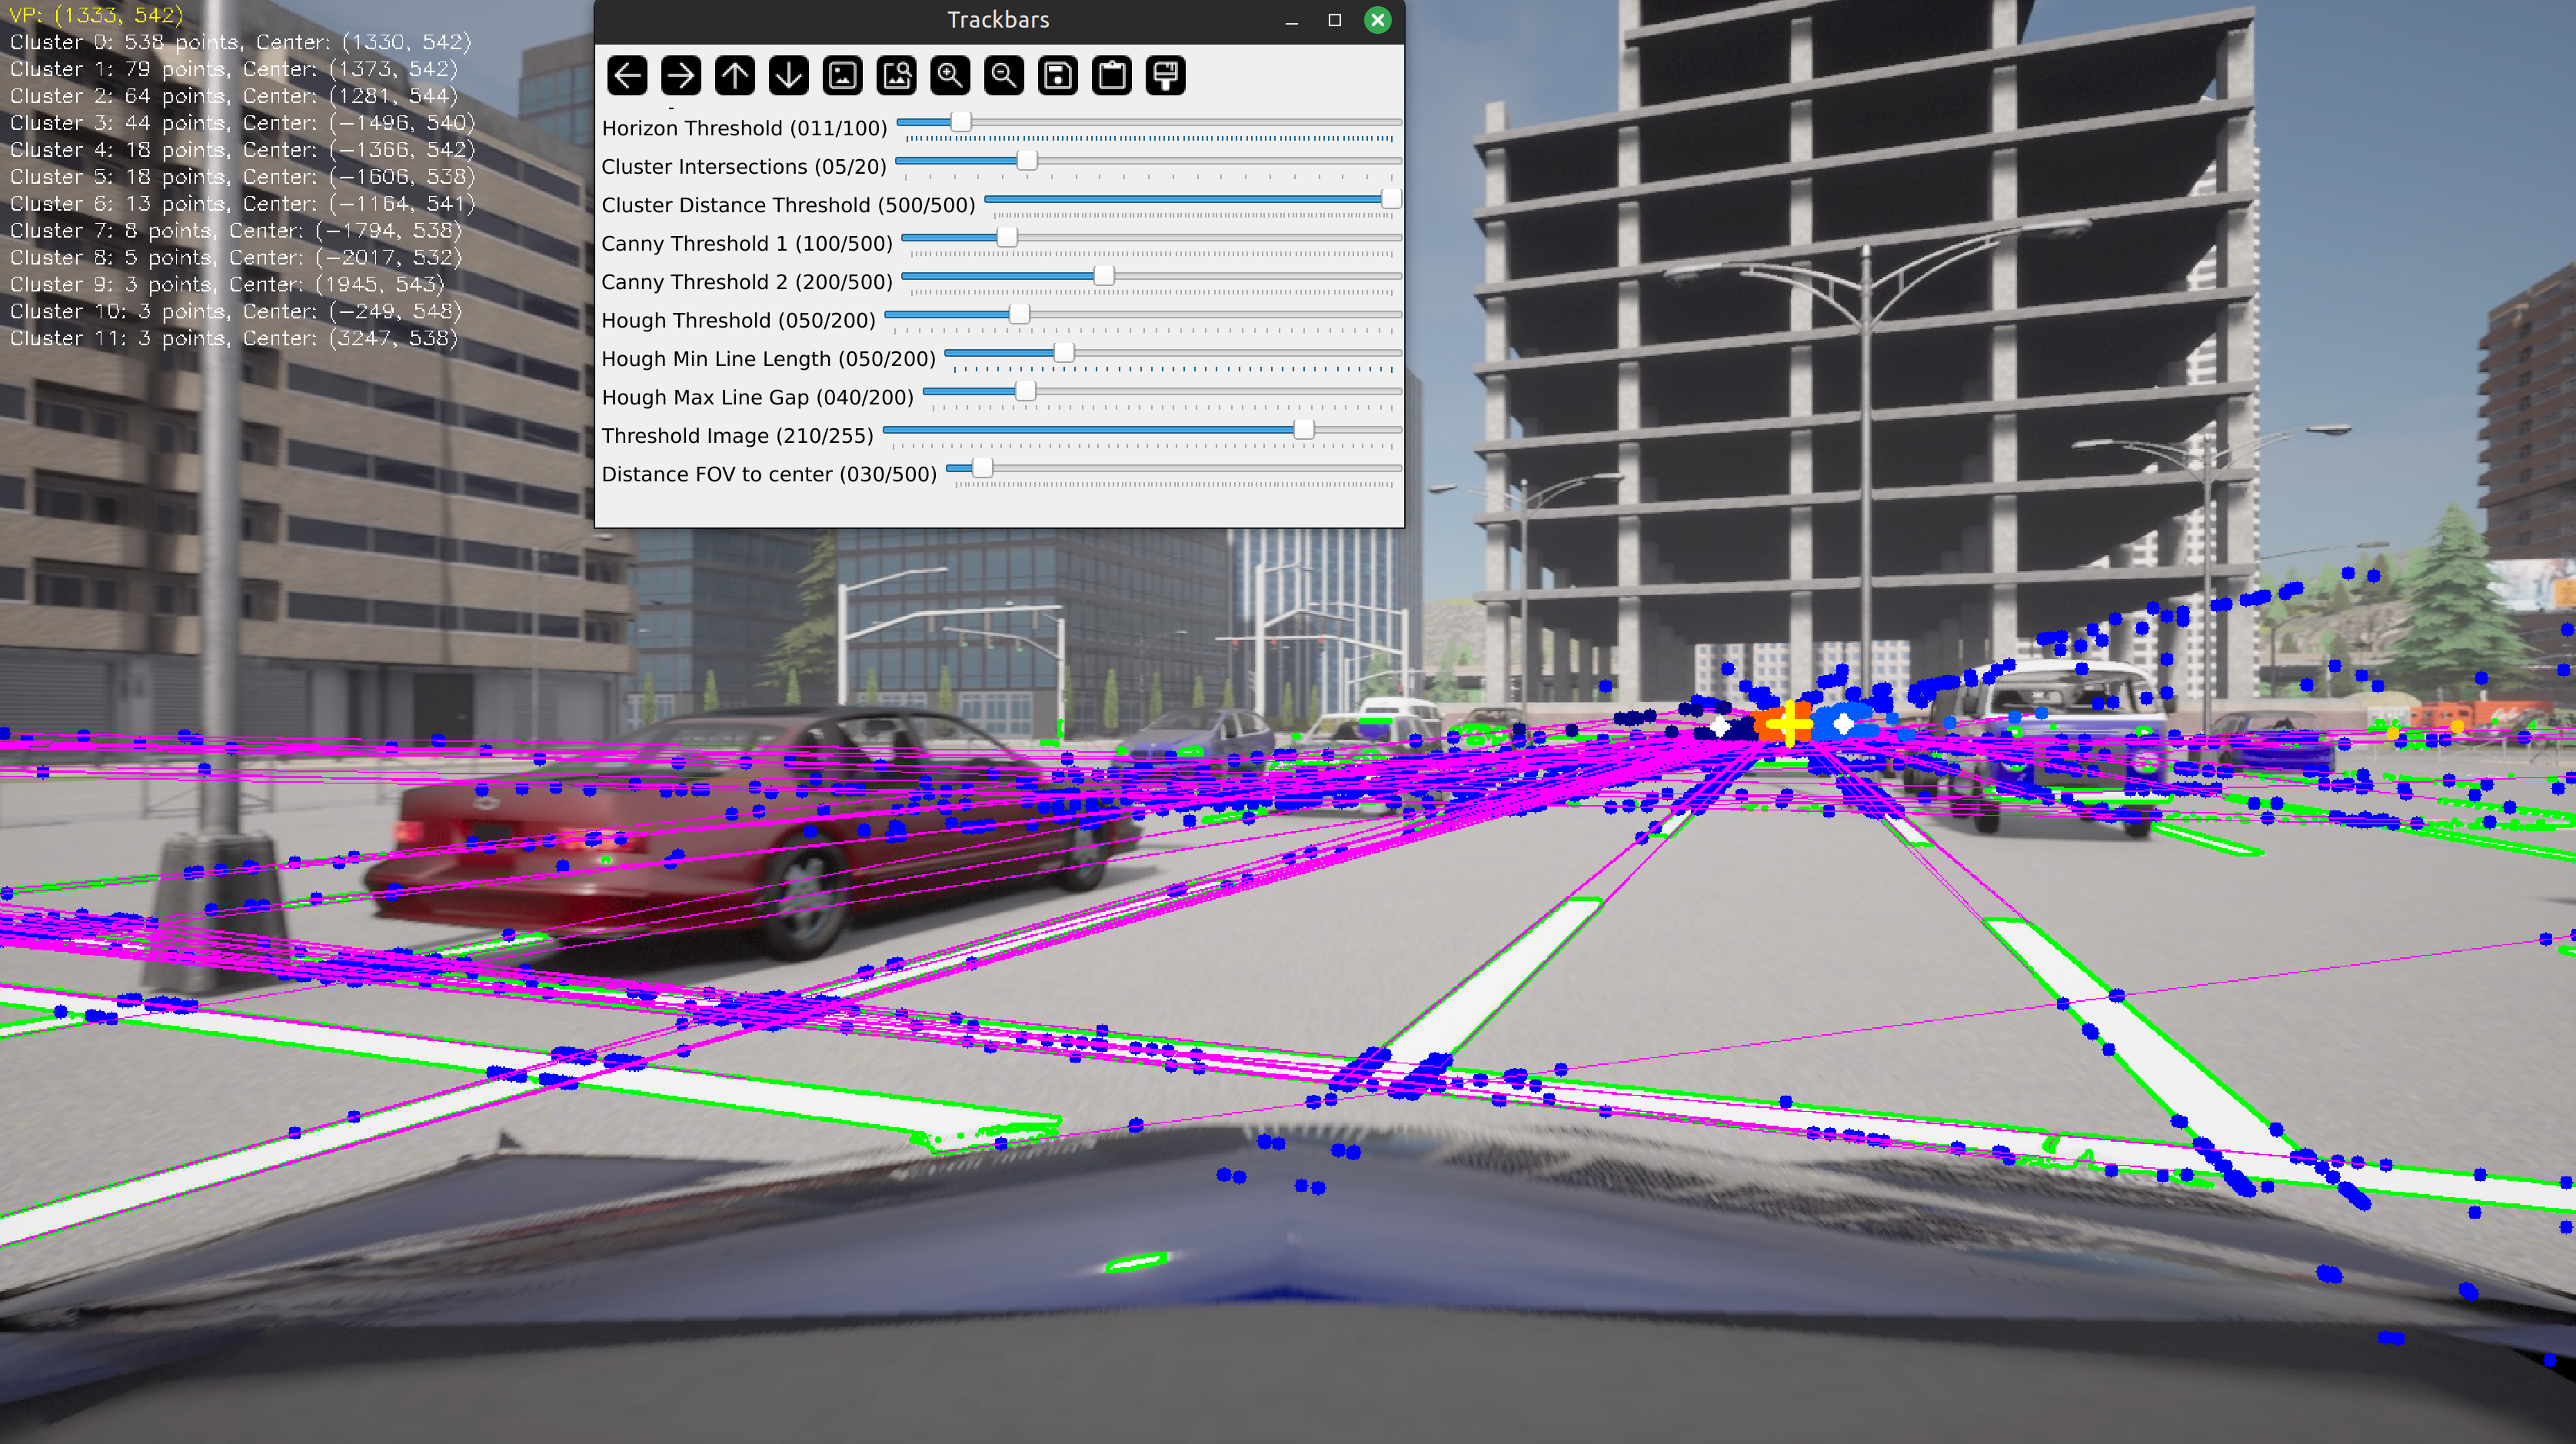
\includegraphics[width=\textwidth]{img/reticule/experimentationRgb}
        \caption{Ejemplo de experimentación (RGB)}
        \label{fig:experimentationRgb}
    \end{subfigure}
    \begin{subfigure}{0.5\textwidth}
        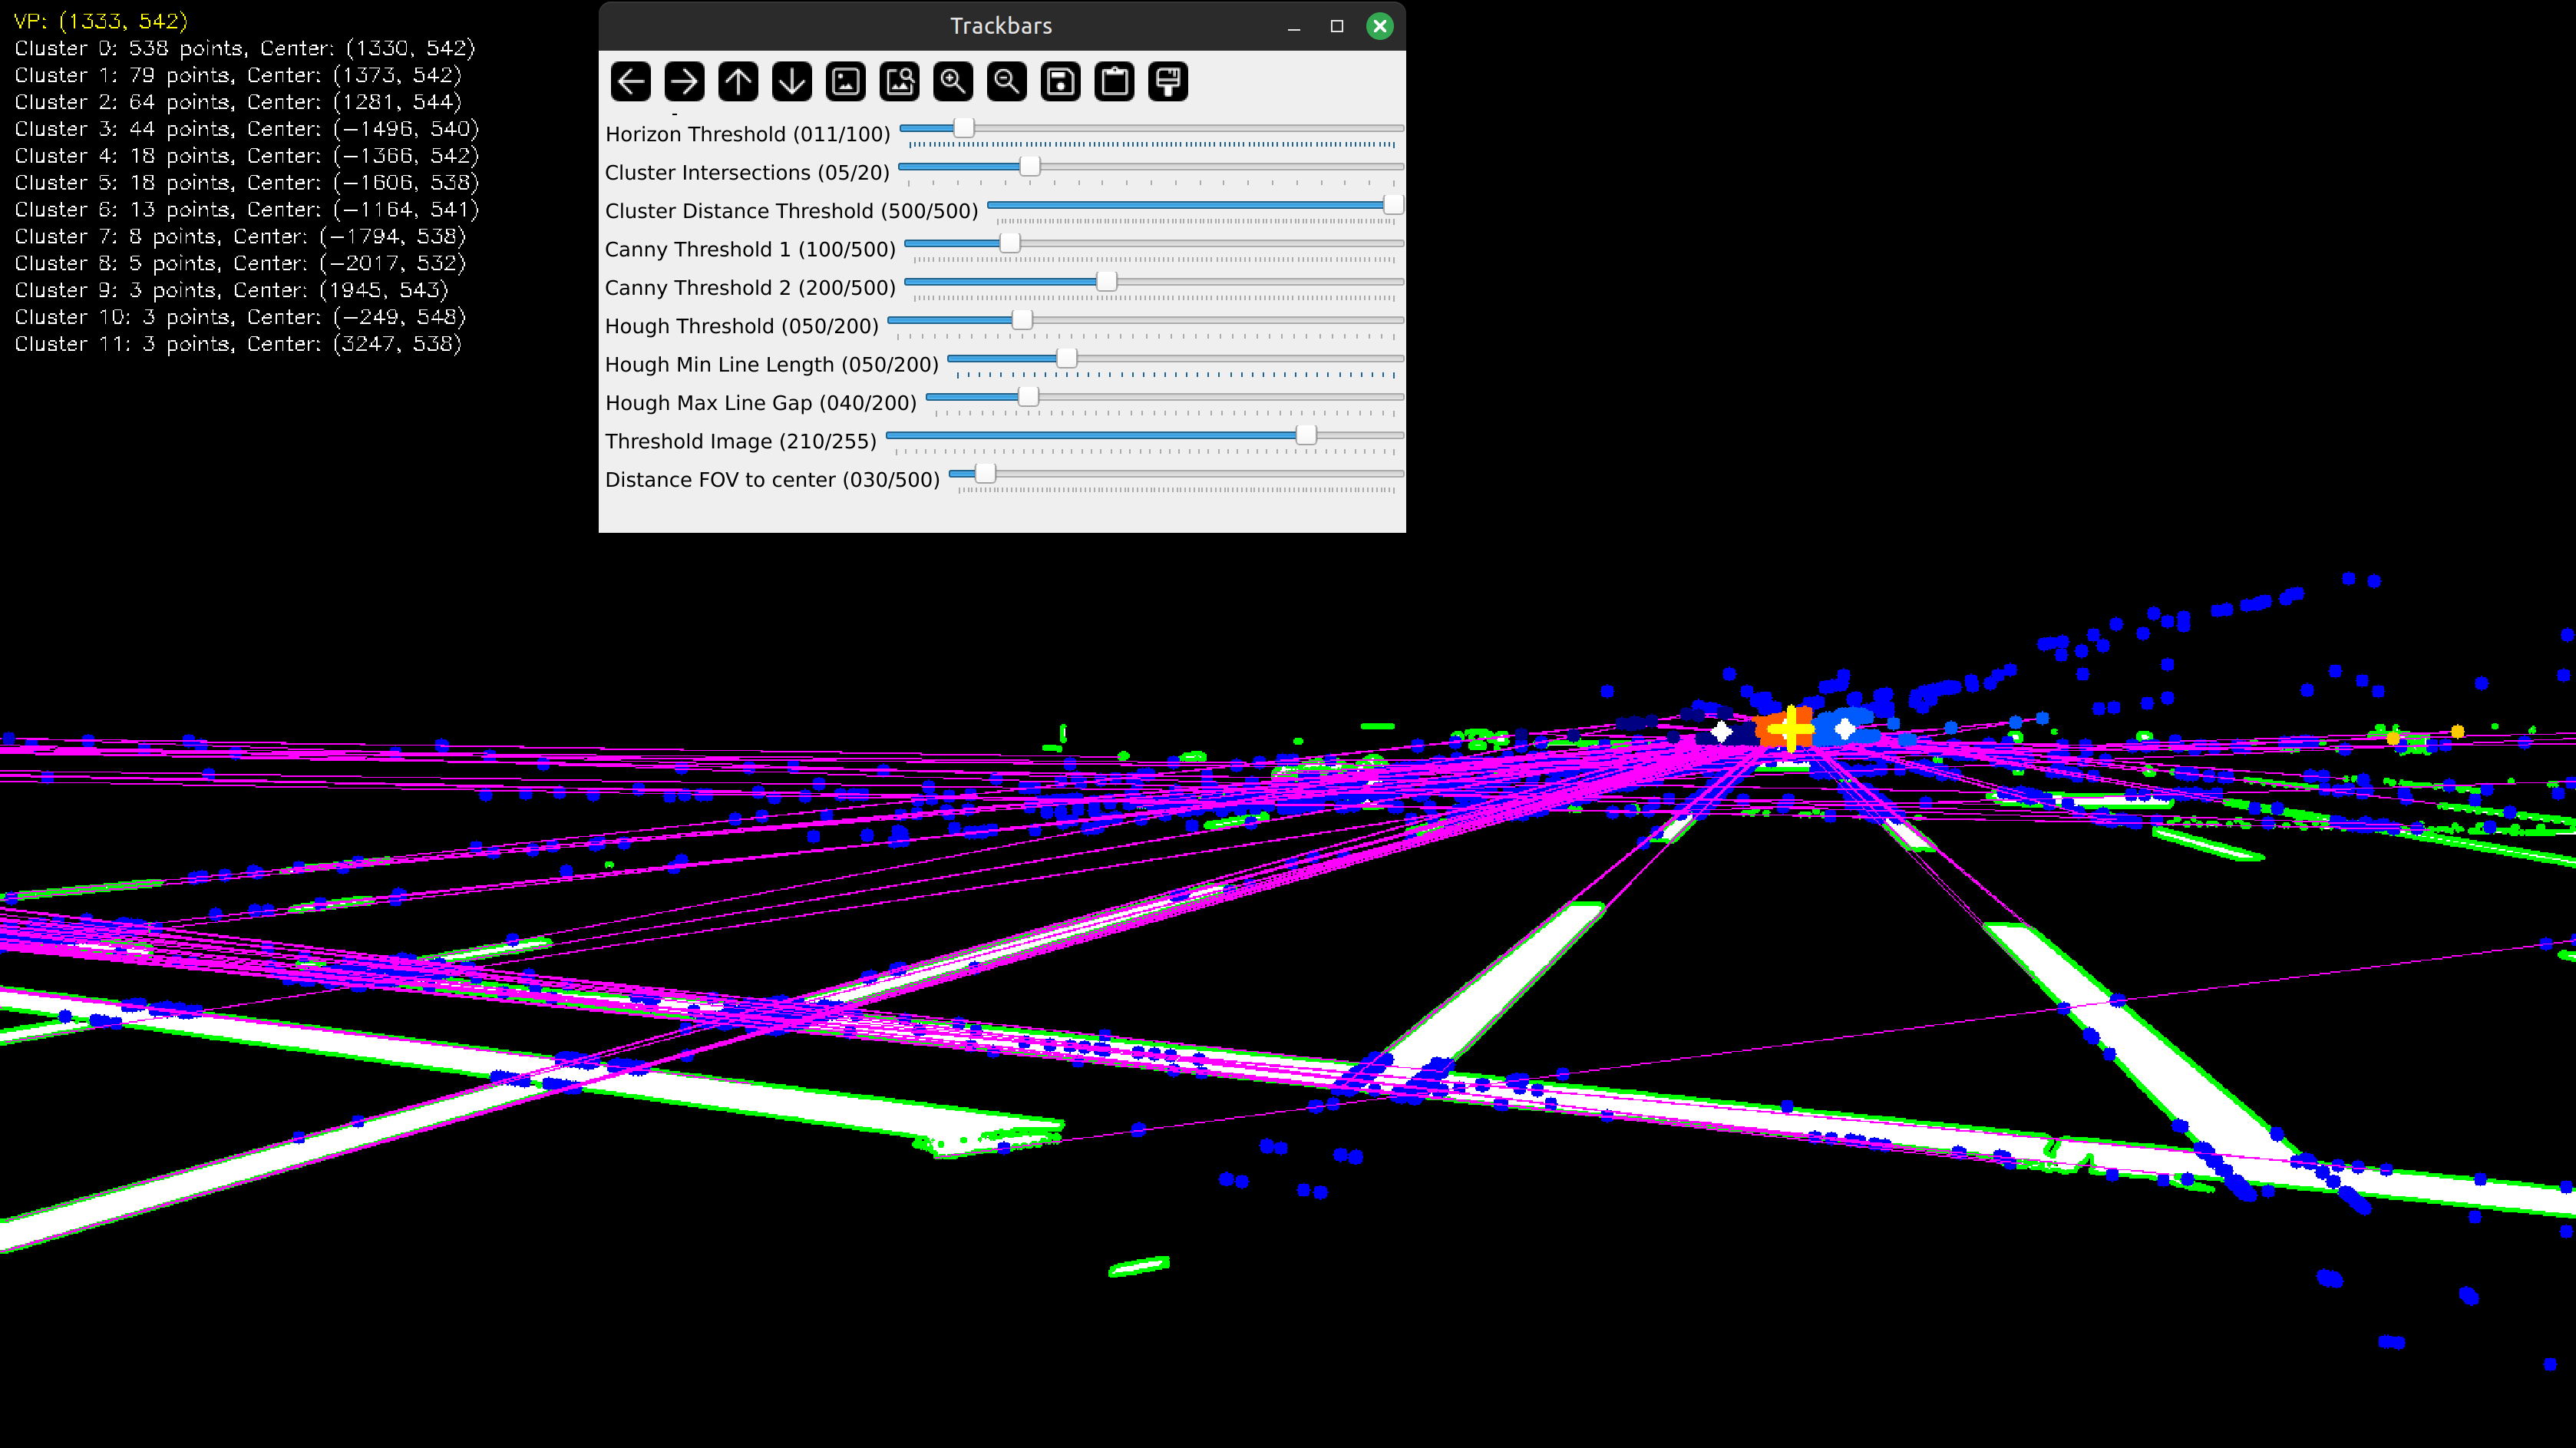
\includegraphics[width=\textwidth]{img/reticule/experimentationBinary}
        \caption{Ejemplo de experimentación (Binaria)}
        \label{fig:experimentationBinary}
    \end{subfigure}
\end{figure}

Cómo se puede observar en la imagen, en el area de Trackbar se muestran los parámetros ajustables y su valor actual,
permitiendo al usuario modificarlos en tiempo real y observar el impacto de estos cambios en la imagen.

    \clearpage


    \section*{Representación de la posición relativa al estacionamiento}
    %! Author = ruben
%! Date = 6/2/2024

% Preamble
\documentclass[11pt]{article}

% Packages
\usepackage{amsmath}

% Document
\begin{document}



\end{document}
    \clearpage

%    \section*{Medición de la posición relativa al estacionamiento en simulación}
%    \section*{Uso de mediciones para parqueo automático}
%    \section*{Experimentos y resultados}
%    \clearpage

    \section*{Cronograma de actividades}
    \begin{center}
    \resizebox{\textwidth}{!}{
        \begin{tabular}{|p{3cm}|*{17}{p{1cm}|}}
            \hline
            \textbf{Actividad} & \multicolumn{17}{c|}{\textbf{Duración}} \\
            \hline
            & Ene & Feb & Mar & Abr & May & Jun & Jul & Ago & Sep & Oct & Nov & Dic
            & Ene & Feb & Mar & Abr & May \\
            \hline
            Investigación y revisión bibliográfica      & \cellcolor{gray!30} & \cellcolor{gray!30} & & & & & & & & & & & & & & & & \\
            \hline
            Diseño y Configuración del Entorno Simulado &                     & \cellcolor{gray!30} & \cellcolor{gray!30} & \cellcolor{gray!30} & & & & & & & & & & & & & & \\
            \hline
            Adquisición y Procesamiento de Datos        &                     &                     &                     &                     & \cellcolor{gray!30} & \cellcolor{gray!30} & \cellcolor{gray!30} & & & & & & & & & & & \\
            \hline
            Desarrollo y Entrenamiento de Algoritmos    &                     &                     &                     &                     &                     &                     & \cellcolor{gray!30} & \cellcolor{gray!30} & \cellcolor{gray!30} &  & & & & & & & & \\
            \hline
            Evaluación y Ajuste del Sistema             &                     &                     &                     &                     &                     &                     &                     & \cellcolor{gray!30} & \cellcolor{gray!30} & \cellcolor{gray!30} & \cellcolor{gray!30} & & & & & & & \\
            \hline
            Documentación y Análisis de Resultados      &                     &                     &                     &                     &                     &                     &                     &                     & \cellcolor{gray!30} & \cellcolor{gray!30} & \cellcolor{gray!30} & \cellcolor{gray!30} & \cellcolor{gray!30} & & & & & \\
            \hline
            Redacción y Revisión del documento de tesis &                     &                     &                     &                     &                     &                     &                     &                     &                     &                     & \cellcolor{gray!30} & \cellcolor{gray!30} & \cellcolor{gray!30} & \cellcolor{gray!30} & \cellcolor{gray!30} & \cellcolor{gray!30} & \cellcolor{gray!30} & \\
            \hline
        \end{tabular}
    }
\end{center}
    \clearpage

    \section*{Estado del arte - Trabajos previos relacionados}
    
\setcounter{secnumdepth}{0}
\noindent
\subsection{
    \textbf{Autonomous Driving Architectures: Insights of Machine Learning and Deep Learning Algorithms}
    ~\cite{bachute2021autonomous}
}\label{subsec:auto-driving-architectures}
El artículo fue publicado en la revista Machine Learning with Applications en 2021 y
proporciona una visión general de la aplicación de algoritmos de Aprendizaje Automático y Aprendizaje Profundo
en sistemas de conducción autónoma, destacando su evaluación en tareas cruciales.
Se destaca el creciente impulso en la investigación de la conducción autónoma debido a sus ventajas inherentes, como la reducción
de la intervención humana y la disociación del conductor del vehículo.
Se subraya la complejidad de estos sistemas,
que involucra la integración de múltiples subsistemas, y se analizan diversas tareas específicas dentro de la conducción autónoma,
como la planificación de movimiento, la detección de peatones y señales de tráfico, el estacionamiento automatizado, entre otras.
El estudio se centra en la aplicación de algoritmos de Aprendizaje Automático y Aprendizaje Profundo para abordar estas tareas,
evaluando y comparando su rendimiento a través de métricas específicas. La investigación ofrece una perspectiva amplia sobre el uso
y la evaluación en el contexto de la conducción autónoma.
\begin{figure}[!ht]
    \begin{subfigure}
        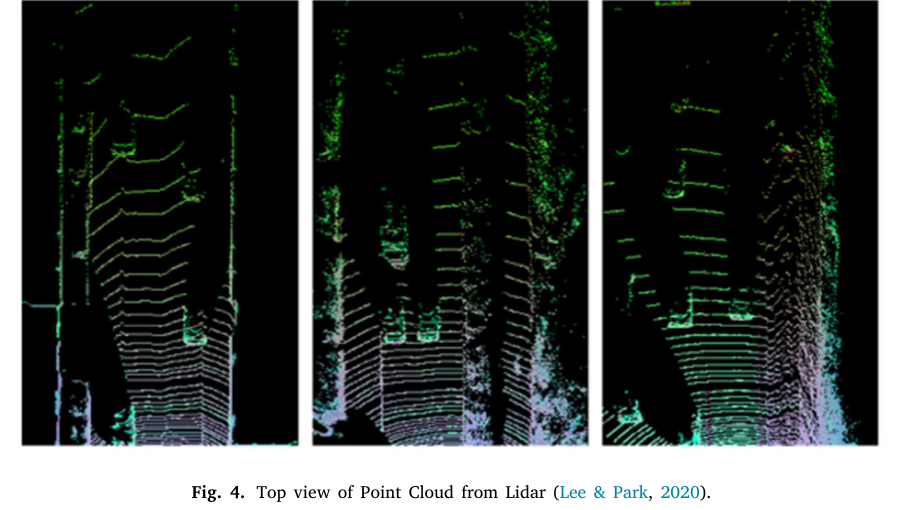
\includegraphics[width=0.5\textwidth]{img/12Screenshot_20231106_142954}\label{fig:12}
    \end{subfigure}
    \begin{subfigure}
        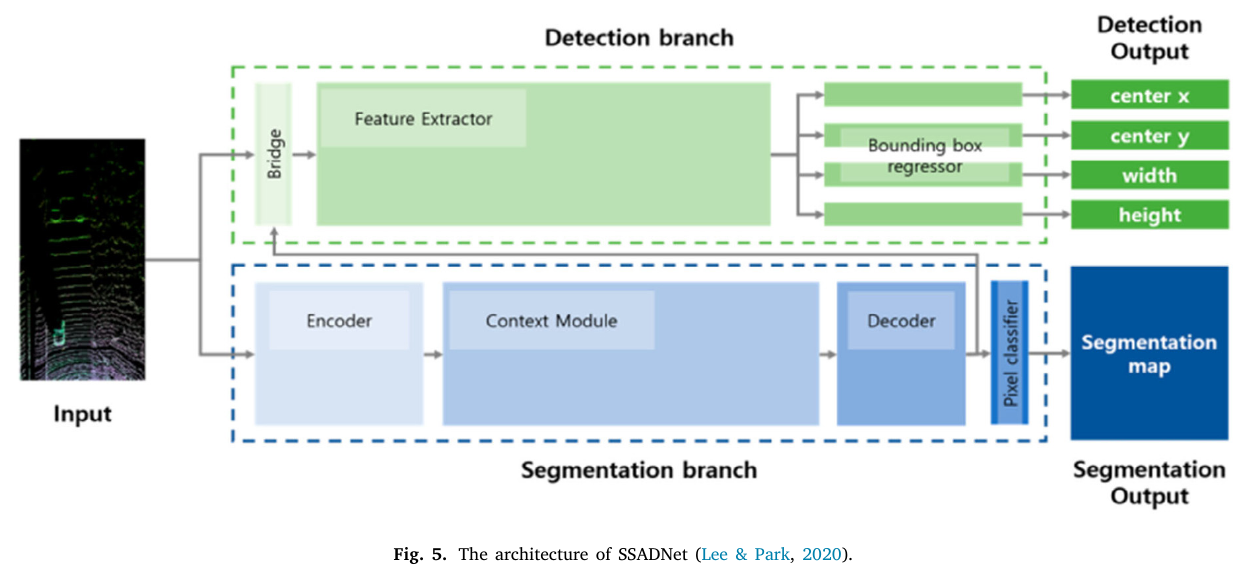
\includegraphics[width=0.5\textwidth]{img/13Screenshot_20231106_143018}\label{fig:13}
    \end{subfigure}
    \begin{subfigure}
        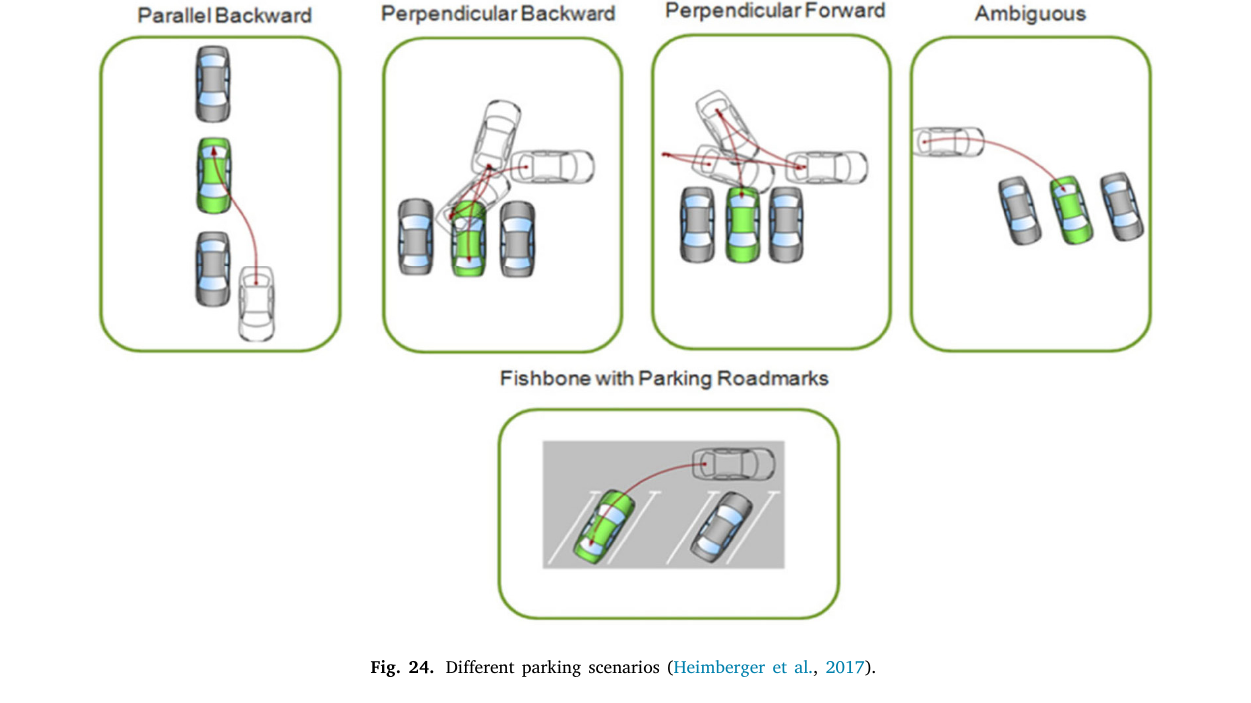
\includegraphics[width=0.5\textwidth]{img/15Screenshot_20231106_143633}\label{fig:15}
    \end{subfigure}
    \begin{subfigure}
        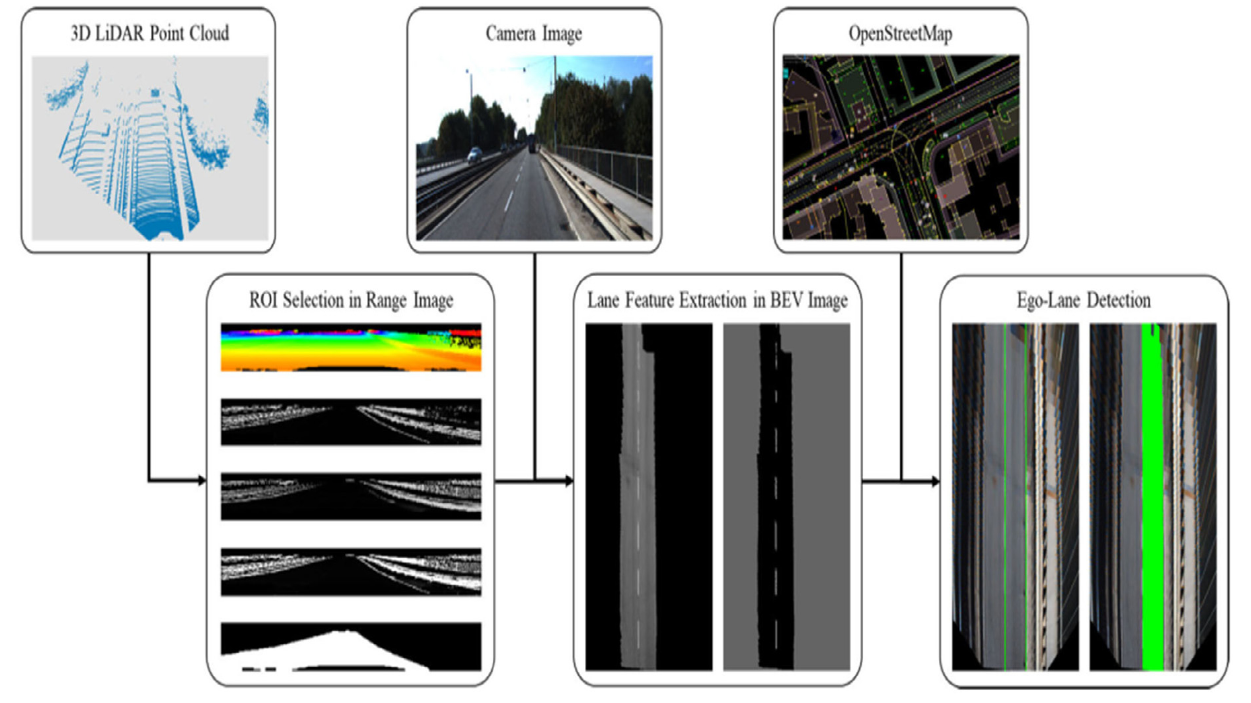
\includegraphics[width=0.5\textwidth]{img/14 Screenshot_20231106_143419}\label{fig:14}
    \end{subfigure}
    \begin{subfigure}
        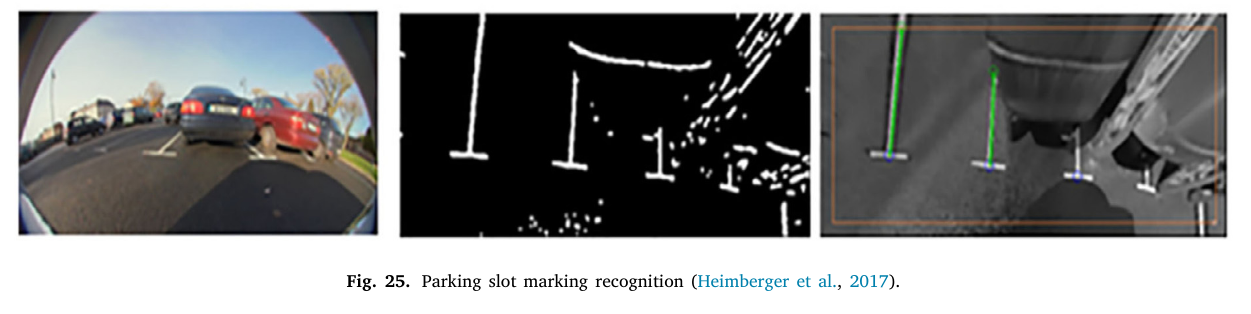
\includegraphics[width=0.99\textwidth]{img/16Screenshot_20231106_143701}\label{fig:16}
    \end{subfigure}
\end{figure}
\clearpage

\subsection{
    \textbf{Vision-based autonomous car racing using deep imitative reinforcement learning}
    ~\cite{cai2021vision}
}\label{subsec:vision-based-autonomous-car-racing}
El artículo fue publicado en la revista IEEE Robotics and Automation Letters en 2021 y aborda el desafío del automovilismo autónomo
en el campo del control robótico, históricamente dependiente de mapas precisos, localización y planificación, lo que lo hace
computacionalmente ineficiente y sensible a cambios en el entorno.
\\
Se destaca el desarrollo de sistemas de aprendizaje profundo de extremo a extremo, que muestran resultados prometedores en la conducción
autónoma.
\\
Sin embargo, estos sistemas suelen basarse en aprendizaje por imitación supervisada (IL), enfrentando problemas de discrepancia
en la distribución de datos.
\\
Aunque se han empleado métodos de aprendizaje por refuerzo (RL), requieren grandes cantidades de datos de interacción riesgosa.
\\
El artículo presenta un enfoque innovador denominado aprendizaje profundo imitativo y de refuerzo (DIRL), que logra la agilidad en
el automovilismo autónomo mediante el uso de entradas visuales.
\\
Este enfoque combina el conocimiento adquirido tanto del aprendizaje por imitación como del aprendizaje basado en modelos de RL,
permitiendo al agente aprender de instructores humanos y mejorar su rendimiento interactuando con un modelo de mundo offline.
La validación del algoritmo se lleva a cabo tanto en simulaciones de conducción de alta fidelidad como en un automóvil RC a escala 1/20 en
el mundo real, con capacidad computacional limitada. \\
Los resultados de la evaluación demuestran que este método supera a enfoques anteriores de IL y RL en eficiencia de muestra y rendimiento
en la tarea, mostrando un gran potencial en el ámbito de la conducción autónoma.
\begin{figure}[!ht]
    \begin{subfigure}
        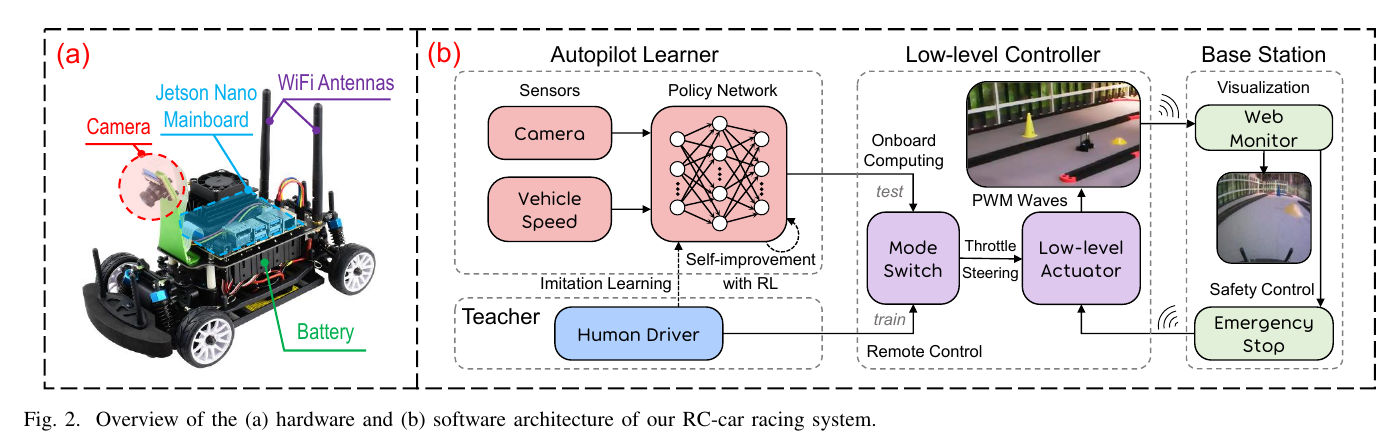
\includegraphics[width=\textwidth]{img/21}\label{fig:21}
    \end{subfigure}
    \begin{subfigure}
        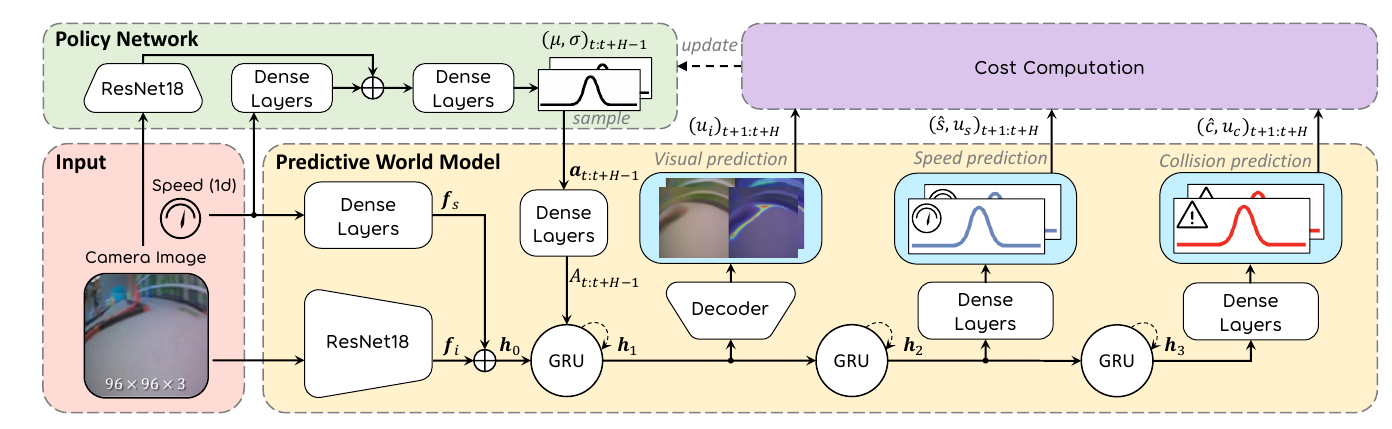
\includegraphics[width=\textwidth]{img/22}\label{fig:22}
    \end{subfigure}
%            \begin{subfigure}
%                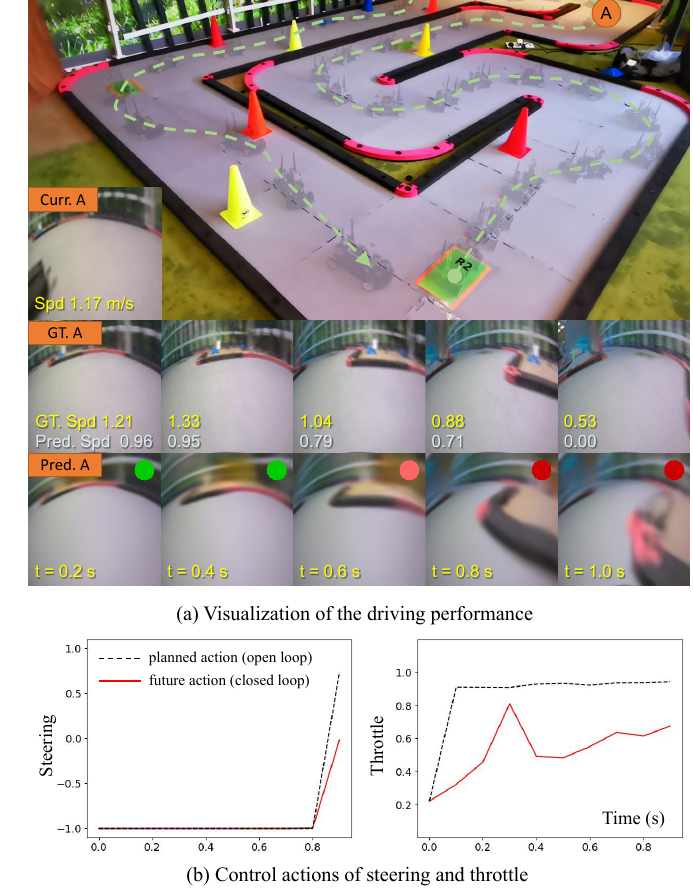
\includegraphics[width=0.2\textwidth]{img/23}\label{fig:23}
%            \end{subfigure}
\end{figure}

\clearpage

\subsection{
    \textbf{Model-based probabilistic collision detection in autonomous driving}
    ~\cite{althoff2009model}
}\label{subsec:probabilistic-collision-detection}
El artículo fue publicado en la revista IEEE Transactions on Intelligent Transportation Systems en 2009 y se centra en la seguridad vial
de los vehículos autónomos en entornos de tráfico complejo.
Su enfoque principal es la detección probabilística de colisiones mediante el análisis y la predicción de la ocupación de la carretera
por parte de otros vehículos.\\
El estudio aborda la incertidumbre inherente en la interacción entre los vehículos autónomos y otros actores del tráfico.
Analiza cómo las mediciones y los posibles comportamientos de estos afectan la predicción de posibles colisiones.
Además, considera las limitaciones en las maniobras de conducción debidas a la geometría de la carretera y la influencia
de estas restricciones en la probabilidad de colisión para trayectorias específicas.\\
Lo más destacado de este enfoque es su eficiencia. La mayor parte de los cálculos intensivos se llevan a cabo offline,
permitiendo disponer de un algoritmo en línea eficiente para aplicaciones en tiempo real.                                                                           \\
Esto contribuye significativamente a la seguridad vial al proporcionar una herramienta precisa y eficaz para la detección anticipada de
posibles colisiones en entornos de conducción autónoma.                                                            \\
\begin{figure}[!ht]
    \begin{subfigure}
        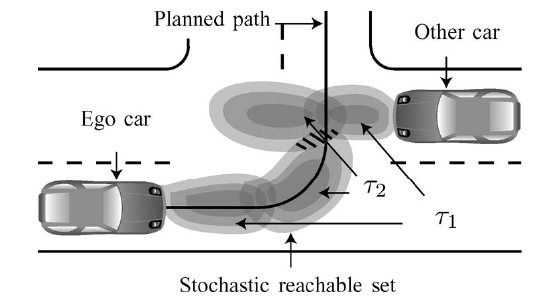
\includegraphics[width=0.5\textwidth]{img/31}\label{fig:31}
    \end{subfigure}
    \begin{subfigure}
        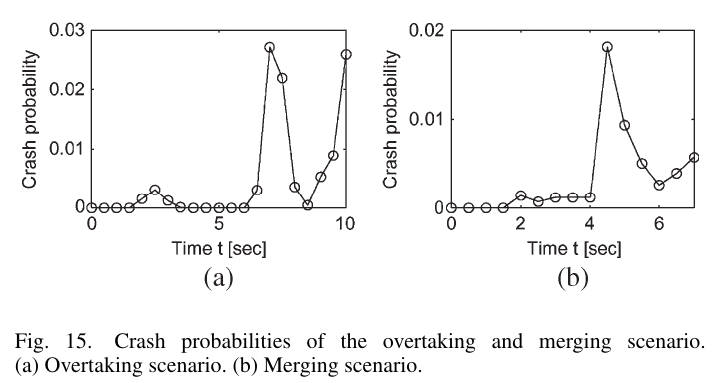
\includegraphics[width=0.5\textwidth]{img/35}\label{fig:35}
    \end{subfigure}
%            \begin{subfigure}
%                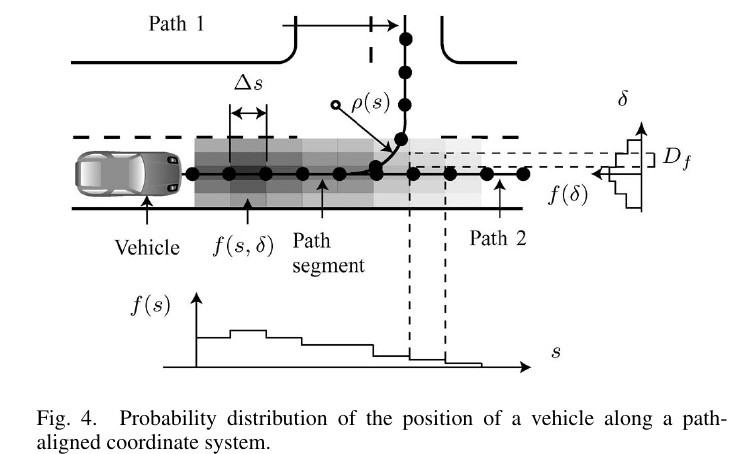
\includegraphics[width=0.5\textwidth]{img/32}\label{fig:32}
%            \end{subfigure}
    \vspace{2cm}
    \begin{subfigure}
        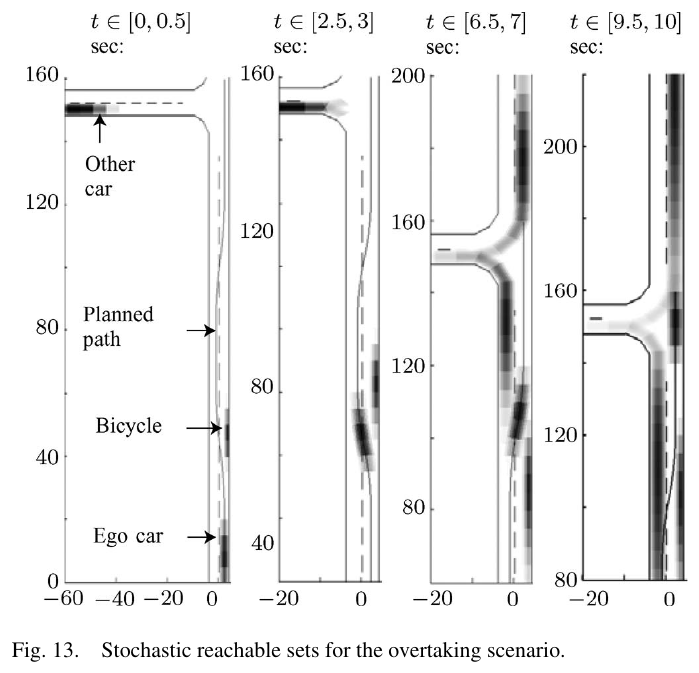
\includegraphics[width=0.5\textwidth]{img/33}\label{fig:33}
    \end{subfigure}
    \begin{subfigure}
        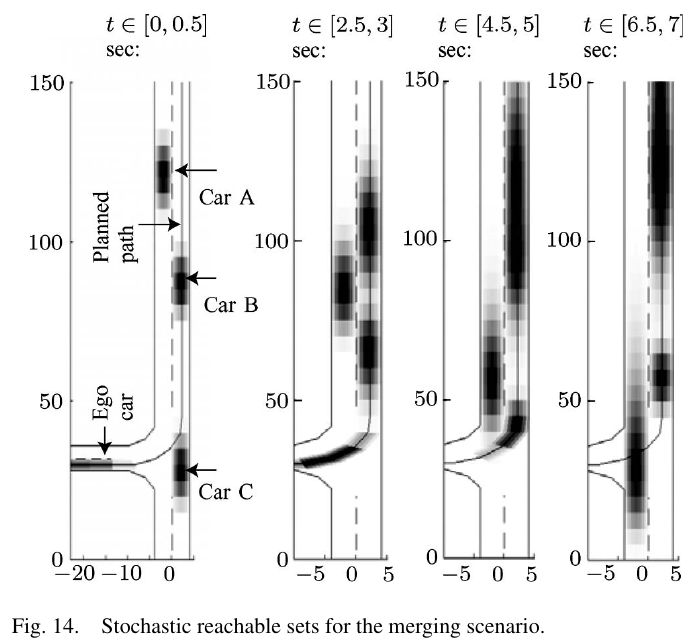
\includegraphics[width=0.5\textwidth]{img/34}\label{fig:34}
    \end{subfigure}

\end{figure}
\clearpage

\subsection{
    \textbf{Vision-based autonomous vehicle systems based on deep learning: A systematic literature review}
    ~\cite{pavel2022vision}
}\label{subsec:vision-based-autonomous-vehicle}
El artículo fue publicado en la revista Applied Science en 2022 y presenta una revisión sistemática de la literatura sobre el empleo
de técnicas de aprendizaje profundo en los sistemas
de vehículos autónomos a lo largo de la última década.                                                                    \\Esta revisión se divide en varios módulos que abarcan distintos aspectos,
desde el análisis de percepción y la toma de decisiones hasta el control, la planificación de trayectorias
y la visualización en sistemas de realidad aumentada tipo HUD.                                                                                                                   \\
Se examinan investigaciones llevadas a cabo entre 2011 y 2021 que se enfocan en la utilización de cámaras RGB como sensores principales
en estos sistemas. Se otorga especial atención a los resultados finales, destacando la visualización en sistemas de realidad aumentada
basados en HUD.                                                                                                      \\Esto incluye advertencias tempranas, marcadores en la carretera para mejorar la navegación y la seguridad, superposición
de información en vehículos y peatones en condiciones visuales extremas para reducir colisiones.
La revisión subraya los métodos actuales de aprendizaje profundo que se basan únicamente en la visión de cámaras RGB, prescindiendo de la
compleja fusión de sensores.                                                                     \\Se espera que este enfoque allane el camino para el desarrollo ágil de sistemas de vehículos autónomos,
siendo prácticos, eficientes y seguros en términos de costos.                                                               \\
\begin{figure}[!ht]
    \begin{subfigure}
        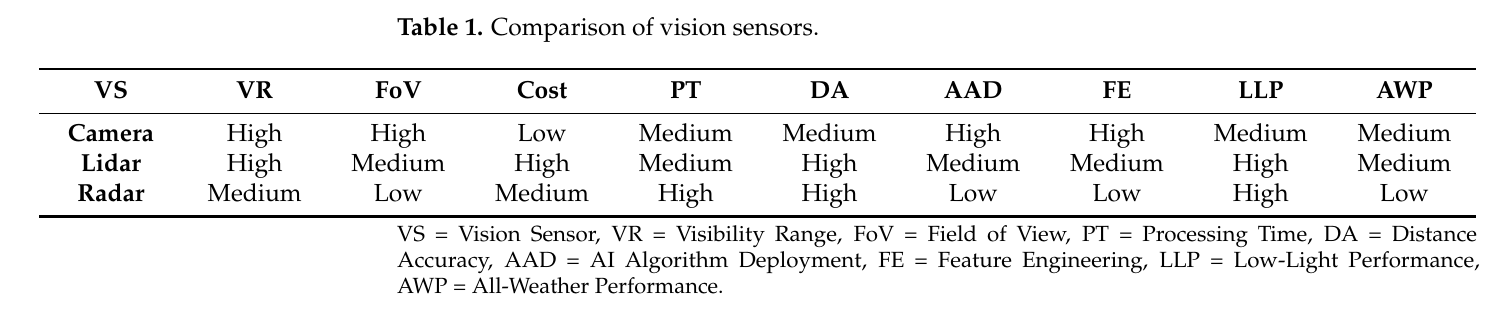
\includegraphics[width=1\textwidth]{img/71}\label{fig:71}
    \end{subfigure}
%            \begin{subfigure}
%                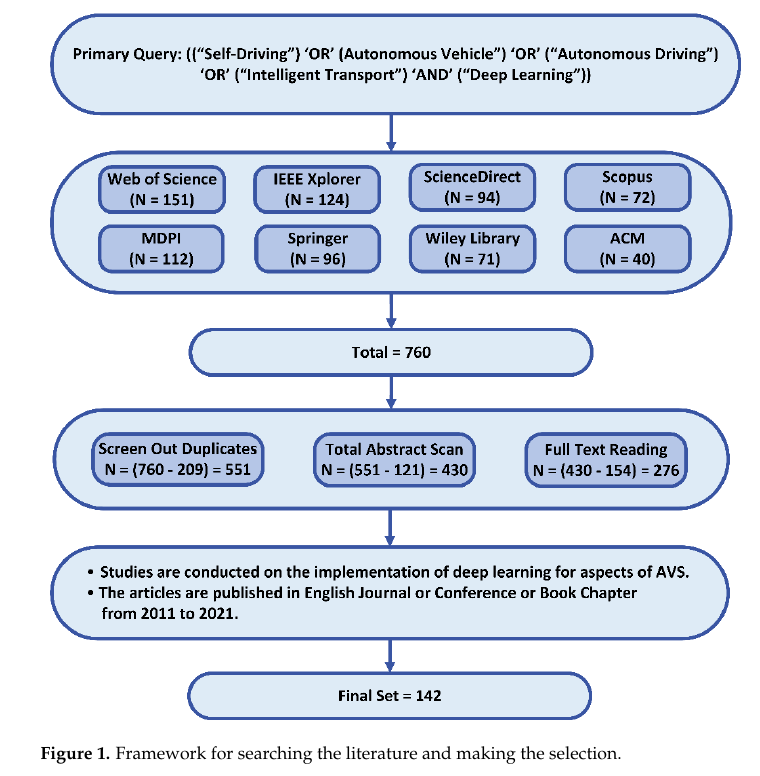
\includegraphics[width=0.5\textwidth]{img/72}\label{fig:72}
%            \end{subfigure}
    \begin{subfigure}
        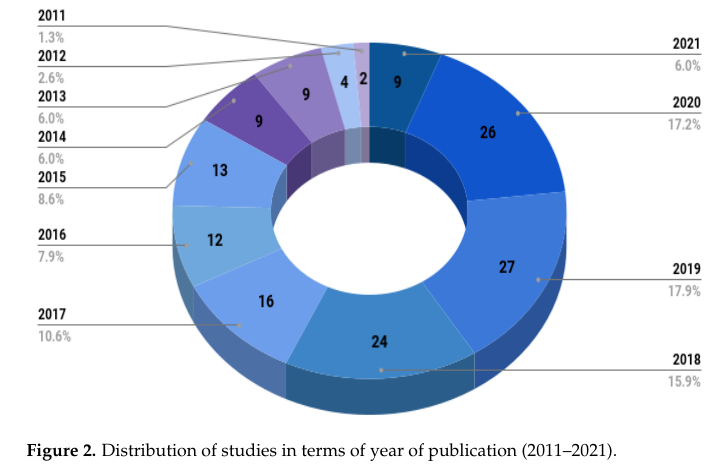
\includegraphics[width=0.5\textwidth]{img/73}\label{fig:73}
    \end{subfigure}
    \begin{subfigure}
        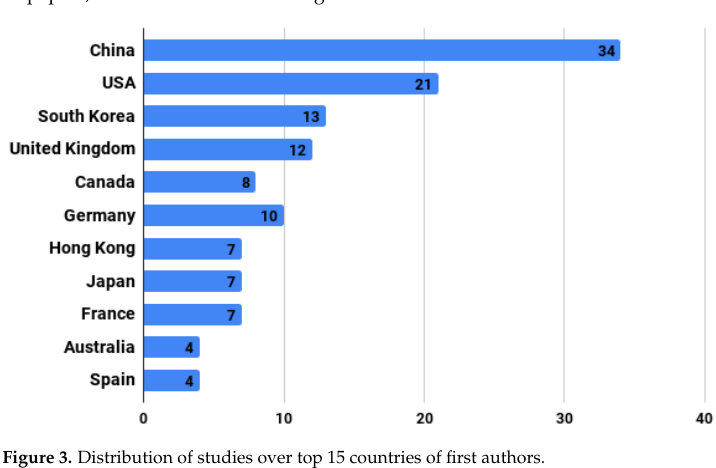
\includegraphics[width=0.5\textwidth]{img/74}\label{fig:74}
    \end{subfigure}
\end{figure}
\clearpage

\subsection{
    \textbf{A cost-effective computer vision-based vehicle detection system}
    ~\cite{alam2022cost}
}\label{subsec:cost-effective-vehicle-detection}
El artículo fue publicado en la revista Concurrent Engineering en 2022 y se enfoca en la detección de vehículos.
\\Destaca la importancia crítica del procesamiento rápido y la detección precisa de vehículos dentro de un sistema autónomo de detección.
\\Presenta un sistema de detección de vehículos basado en visión por computadora que utiliza un algoritmo de Gentle Adaptive Boosting
con características tipo Haar para generar hipótesis de vehículos de manera eficiente.
Para abordar los errores potenciales, propone el uso de un algoritmo de Máquinas de Vectores de Soporte (SVM) entrenado con características
del histograma de gradientes orientados (HOG) para filtrar las hipótesis falsas.
\\El descriptor HOG se centra en la forma y contornos de los vehículos, mejorando la precisión de la detección.
La combinación de características tipo Haar y HOG permite cumplir los objetivos de detección en la conducción autónoma.
\\El rendimiento del sistema propuesto se evalúa con imágenes capturadas durante el día y la noche y se compara con tres detectores
de vehículos existentes. Los resultados muestran una precisión promedio del 0.97 para imágenes capturadas durante el día
y del 0.94 para imágenes nocturnas.                                                                                               \\Además, se destaca que el sistema propuesto requiere aproximadamente 15 veces menos tiempo
de entrenamiento en comparación con las técnicas existentes, utilizando la misma cantidad de datos de imágenes y la misma unidad
de procesamiento central (CPU). Esto demuestra una mejora significativa en la eficiencia del sistema propuesto en términos de tiempo de entrenamiento.
\begin{figure}[!ht]
%            \begin{subfigure}
%                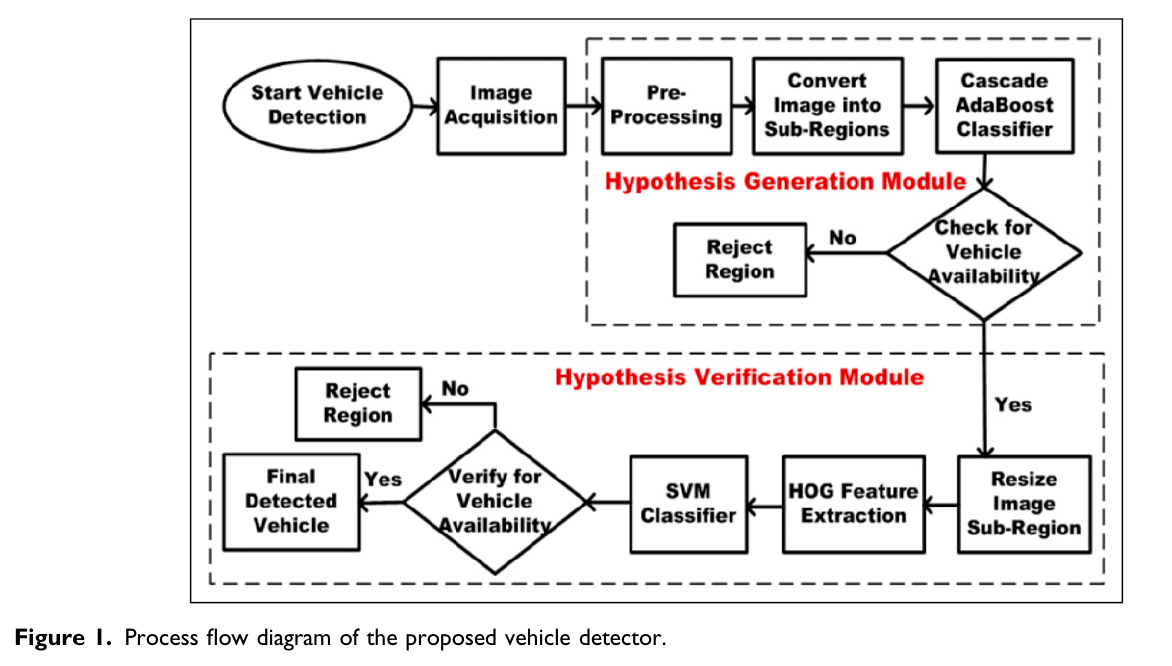
\includegraphics[width=0.6\textwidth]{img/81}\label{fig:81}
%            \end{subfigure}
%            \begin{subfigure}
%                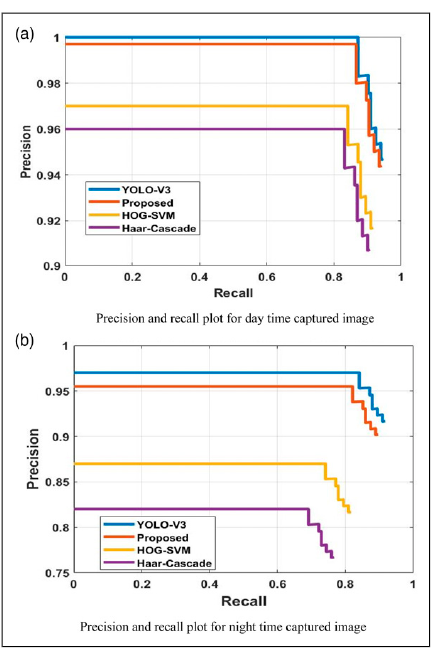
\includegraphics[width=0.5\textwidth]{img/86}\label{fig:82}
%            \end{subfigure}
    \begin{subfigure}
        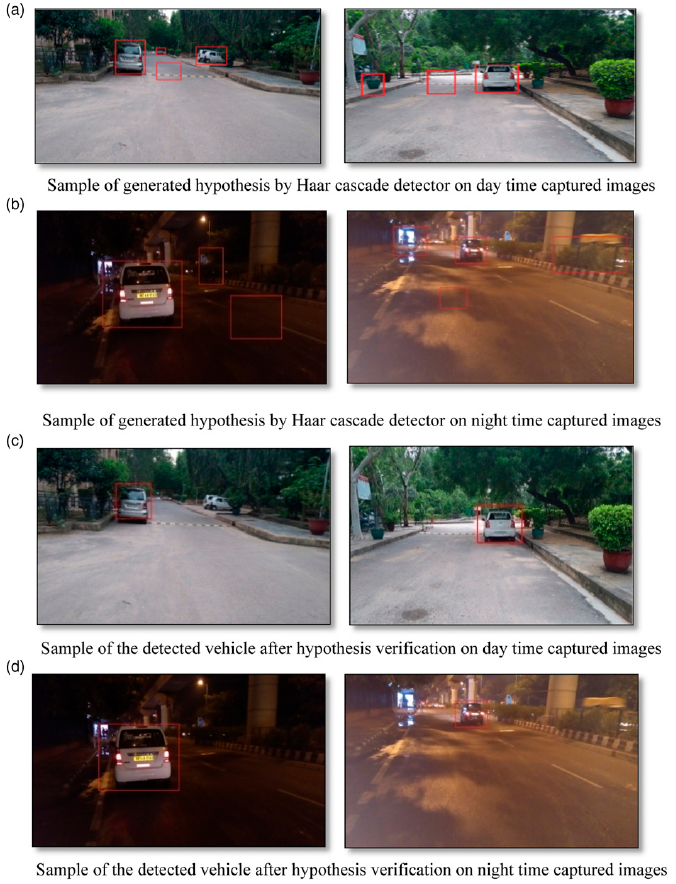
\includegraphics[width=0.5\textwidth]{img/84}\label{fig:84}
    \end{subfigure}
    \begin{subfigure}
        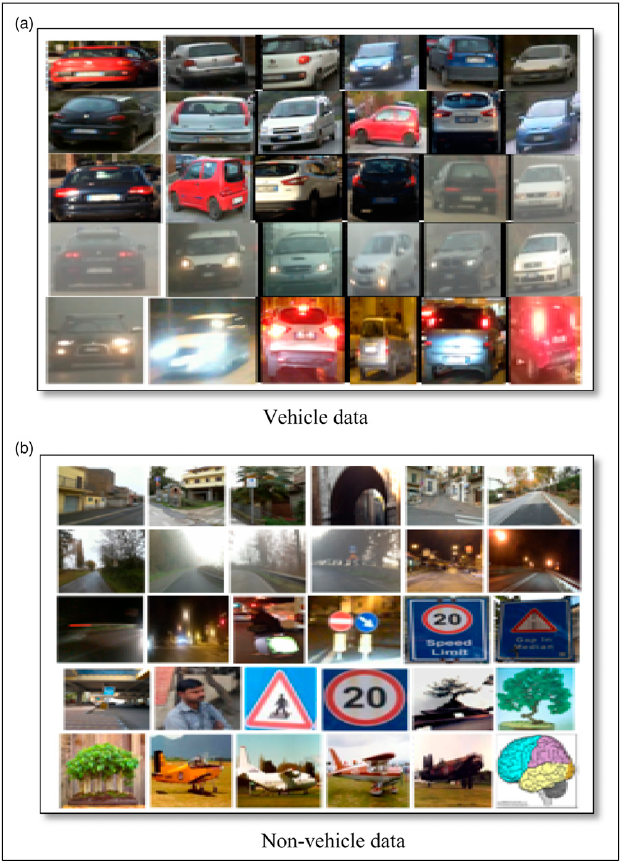
\includegraphics[width=0.5\textwidth]{img/82}\label{fig:86}
    \end{subfigure}
\end{figure}
\clearpage


    \section*{Tabla comparativa}
    \begin{center}
    \resizebox{\textwidth}{!}{
        \begin{tabular}{|p{5cm}|p{2cm}|p{2cm}|p{2cm}|p{2cm}|p{2cm}|p{2cm}|}
            \hline
            \textbf{Características}
            & \textbf{Propia}
            & \textbf{Autonomous Driving Architectures \cite{bachute2021autonomous}}
            & \textbf{Vision-based Autonomous Car Racing \cite{cai2021vision}}
            & \textbf{Model-based Probabilistic Collision Detection \cite{althoff2009model}}
            & \textbf{Vision-based Autonomous Vehicle Systems \cite{pavel2022vision}}
            & \textbf{Cost-effective Vehicle Detection System \cite{alam2022cost}} \\
            \hline
            Uso de algoritmos de Aprendizaje Automático y Aprendizaje Profundo & X & X &   &   & X &   \\
            \hline
            Enfoque en la conducción autónoma                                  & X & X & X & X & X & X \\
            \hline
            Ventajas de la conducción autónoma                                 & X & X &   &   &   &   \\
            \hline
            Complejidad de los sistemas de conducción autónoma                 &   & X &   &   &   &   \\
            \hline
            Análisis de tareas en la conducción autónoma                       & X & X &   &   &   &   \\
            \hline
            Evaluación y comparación de algoritmos                             &   & X & X &   &   &   \\
            \hline
            Predicción estocástica de ocupación de la carretera                &   &   &   & X &   &   \\
            \hline
            Eficiencia en cálculos intensivos                                  &   &   & X & X &   &   \\
            \hline
            Utilización de cámaras RGB como sensores principales               & X &   & X &   & X &   \\
            \hline
            Detección de vehículos en conducción autónoma                      & X &   &   &   &   & X \\
            \hline
        \end{tabular}
    }
\end{center}
    \clearpage

    \section*{Referencias bibliográficas}
    \bibliographystyle{acm}
    \bibliography{referecias}

\end{document}
